\documentclass[11pt,dvipsnames]{report} % {{{
\usepackage[spanish]{babel}
\usepackage[utf8]{inputenc}
\usepackage[T1]{fontenc}
\usepackage{makeidx}
\usepackage{graphicx}
\usepackage{subfig}
\usepackage{amsmath}
\usepackage{amsfonts}
\usepackage{amssymb}
\usepackage{amsthm}
\usepackage{authblk} % para la manipulación de autores y afiliación
\usepackage[pdftex]{hyperref}
\usepackage{multirow}
\usepackage{multicol}
\usepackage{float}
\usepackage{xcolor}
\usepackage{booktabs}
\usepackage{colortbl}
\usepackage{bbold}
\usepackage{physics}
\usepackage{mathtools}
\usepackage{dsfont}
\usepackage{tensor}

% Theorems, proofs, etc
\usepackage{amsthm}



% triangulo
\usepackage{pifont}
\usepackage{fontawesome5}
\hypersetup{
    colorlinks=true,    % Enlaces con color en vez de cuadros
    linkcolor=red,      % Color de los enlaces internos (citas)
    citecolor=red,      % Color de las citas
    filecolor=blue,     % Color de los enlaces a archivos
    urlcolor=blue       % Color de los enlaces externos (URLs)
}
\usepackage{caption}
\usepackage{tcolorbox}
\newcommand{\partition}{\mathfrak{z}}
\newcommand{\bigpartition}{\mathcal{Z}}
\newcommand{\N}{\mathbb{N}}
\newcommand{\Z}{\mathbb{Z}}
\newcommand{\Q}{\mathbb{Q}}
\newcommand{\I}{\mathbb{I}}
\newcommand{\R}{\mathbb{R}}
\newcommand{\C}{\mathbb{C}} %Conjuntos numericos
\newcommand{\F}{\mathbb{F}} %Campo Cualquiera
\newcommand{\Pos}{\mathbb{P}} %Reales positivos
\newcommand{\hilbert}{\mathcal{H}} % Espacio de Hilbert
\newcommand{\f}{\textit{f}} %f de funcion
\newcommand{\g}{\textit{g}}
\newcommand{\kernel}{\mathscr{N}} %kernel
\newcommand{\range}{\mathcal{R}} %range
\newcommand{\lagran}{\mathcal{L}} %lagrangiano
\newcommand{\laplace}{\mathscr{L}} %transformada de laplace, mapas lineales
\newcommand{\inner}[2]{\langle #1 , #2 \rangle}
\newcommand{\metric}[2]{\rho(#1,#2)}
\newcommand{\psim}{\overset{\sim}{\psi}}
\newcommand{\pauli}[1]{\sigma _{#1}}
\newcommand{\updownarrows}{\uparrow \downarrow}
\newcommand{\downuparrows}{\downarrow \uparrow}





\usepackage{fancybox}
\usepackage{colortbl}
\usepackage{amsbsy}
\usepackage[draft,inline,nomargin]{fixme} \fxsetup{theme=color}

%This defines my comments
\definecolor{mycolor}{RGB}{255,0,0}
\FXRegisterAuthor{ds}{sds}{\color{mycolor}DS}


\usepackage[]{lineno} 
%\linenumbers
%\setlength\linenumbersep{3pt}

\newcommand{\fref}[1]{fig.~\ref{#1}}  \newcommand{\tref}[1]{table~\ref{#1}}
\newcommand{\Fref}[1]{Fig.~\ref{#1}}  \newcommand{\Tref}[1]{Table~\ref{#1}}

\usepackage{hyperref}
%\usepackage{commath}
\decimalpoint
\renewcommand{\tablename}{Tabla}
\oddsidemargin 0in
\textwidth 6.5in
\topmargin -0.5in
\textheight 8.5in

\newcommand{\psii}{\psi_i}
\newcommand{\Pk}[1]{\ket{\psi_{#1} }}
\newcommand{\Pb}[1]{\bra{\psi_{#1} }}
\newcommand{\pk}{\ket{\psi}}
\newcommand{\pkt}{\ket{\psi (t)}}
\newcommand{\M}{\mathcal{M}^{(N)}}
\newcommand{\E}{\mathcal{E}}
\newcommand{\Erho}{\mathcal{E}(\rho)}
\newcommand{\1}{\mathds{1}}
\newcommand{\ten}{\otimes}
\newcommand{\h}[1]{\colorbox{Yellow}{#1}}
\newcommand{\hi}{\mathcal{H}}
\newcommand{\tx}[1]{\text{#1}}
\newcommand{\here}{\h{\hspace{15cm}} }
\newcommand{\rhoi}{\dyad{\psii}{\psii}}
\newcommand{\ind}[2]{{{}^{#1}_{#2}}}
\newcommand{\QH}{\abs{Q_H}}
\newcommand{\QL}{\abs{Q_L}}
\newcommand{\W}{\abs{W}}
\newcommand{\uv}[1]{\vb{\hat{#1}}}
\newcommand{\ep}{\epsilon_0}
\renewcommand{\L}{\mathcal{L}}
\newcommand{\spinp}[1]{\ket{S_{#1} ,+}}
\newcommand{\spinm}[1]{\ket{S_{#1} ,-}}
\newcommand{\plus}{\ket{+}}
\newcommand{\minus}{\ket{-}}

\renewcommand{\uv}[1]{\boldsymbol{\hat{\mathrm{#1}}}}
\renewcommand{\d}{\mathrm{d}}


\def\dbar{{\mathchar'26\mkern-12mu d}}


% Para que funcione mejor la numeración {{{
% https://tex.stackexchange.com/questions/43648/why-doesnt-lineno-number-a-paragraph-when-it-is-followed-by-an-align-equation
%\newcommand*\patchAmsMathEnvironmentForLineno[1]{%
%  \expandafter\let\csname old#1\expandafter\endcsname\csname #1\endcsname
%  \expandafter\let\csname oldend#1\expandafter\endcsname\csname end#1\endcsname
%  \renewenvironment{#1}%
%     {\linenomath\csname old#1\endcsname}%
%     {\csname oldend#1\endcsname\endlinenomath}}% 
%\newcommand*\patchBothAmsMathEnvironmentsForLineno[1]{%
%  \patchAmsMathEnvironmentForLineno{#1}%
%  \patchAmsMathEnvironmentForLineno{#1*}}%
%\AtBeginDocument{%
%\patchBothAmsMathEnvironmentsForLineno{equation}%
%\patchBothAmsMathEnvironmentsForLineno{align}%
%\patchBothAmsMathEnvironmentsForLineno{flalign}%
%\patchBothAmsMathEnvironmentsForLineno{alignat}%
%\patchBothAmsMathEnvironmentsForLineno{gather}%
%\patchBothAmsMathEnvironmentsForLineno{multline}%
%}
% }}}
% }}}


%%%%%%%%%
\newcommand*\patchAmsMathEnvironmentForLineno[1]{%
  \expandafter\let\csname old#1\expandafter\endcsname\csname #1\endcsname
  \expandafter\let\csname oldend#1\expandafter\endcsname\csname end#1\endcsname
  \renewenvironment{#1}%
     {\linenomath\csname old#1\endcsname}%
     {\csname oldend#1\endcsname\endlinenomath}}%
\newcommand*\patchBothAmsMathEnvironmentsForLineno[1]{%
  \patchAmsMathEnvironmentForLineno{#1}%
  \patchAmsMathEnvironmentForLineno{#1*}}%
\AtBeginDocument{%
  \patchBothAmsMathEnvironmentsForLineno{equation}%
  \patchBothAmsMathEnvironmentsForLineno{align}%
  \patchBothAmsMathEnvironmentsForLineno{flalign}%
  \patchBothAmsMathEnvironmentsForLineno{alignat}%
  \patchBothAmsMathEnvironmentsForLineno{gather}%
  \patchBothAmsMathEnvironmentsForLineno{multline}%
}
%%%%%%%%%


\title{Notas de estudio para Examen Privado\\
Licenciatura en Física}
\author{Diego Sarceño}

\newtheorem{definition}{Definición}[section]

\newtheorem{teorema}{Teorema}[section]

\newtheorem{property}{Propiedad}[section]

\begin{document}
\maketitle

\tableofcontents


\chapter{Termodinámica}

\textit{La termodinámica es el estudio de las restricciones a las posibles propiedades de la materia que se derivan de las propiedades de simetría de las leyes fundamentales de la física.}

\section{Conceptos Básicos}

\paragraph{Propósito: } La termodinámica busca describir sistemas de muchas partículas ($10^{23}$ típicamente). Gases, líquidos, cristales, estrellas, universo, \ldots ,  \underline{sistemas macroscópicos} y en particular, estudiar los procesos de transferencia de energía (trabajo y calor) entre cuerpos macroscópicos\footnote{Más adelante se tratará la parte microscópica con la Mecánica Estadística, poder explicativo y predictivo sobre propiedades macroscópicas de la materia, partiendo de una descripción microscópica.}. 

\begin{itemize}
	\item Definir cantidades físicas, "variables de estado" que caracterizan un sistema macroscópico: $V,T,N,U,\ldots$.
	\item Relacionar estas cantidades entre sí:
		\begin{enumerate}
			\item Válidas para cualquier sistema en equilibrio:
			\begin{enumerate}
				\item Leyes axiomáticas de la termodinámica, como Ley de la Energía, Ley de la Entroía, etc.
			\end{enumerate}
			\item Específicas
			\begin{enumerate}
				\item Por ecuaciones de estado como: fenomenológicas, empíricas, experimentales en la mayoria de los casos.
			\end{enumerate}
		\end{enumerate}
\end{itemize}


Es importante mencionar que la termodinámica clásica macroscópica no puede explicar porqué una ecuación de estado describe un sistema partícular.



\section{Sistemas Termodinámicos y Cantidades de Estado}

\begin{enumerate}
	\item Sistema Termodinámico:
	\begin{figure}[H]
		\centering
		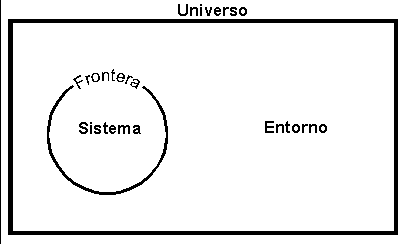
\includegraphics[scale=0.3]{./img/thermodynamicSystem.png}
		\label{thermodynamicSystem}
		\caption{Representación gráfica de las partes de un sistema termodinámico.}
	\end{figure}
	
	\item Tipos de Sistemas: (depende de la frontera)
	\begin{itemize}
		\item Sistemas aislados: No intercambian energía con el entorno.
		\item Sistemas cerrados
	\end{itemize}
\end{enumerate}







\part{Mecánica Estadística}


\vspace*{\fill}

\begin{center}
	\textit{Ludwig Boltzmann, quien dedicó gran parte de su vida a estudiar Mecánica Estadística, murió en 1906, por su propia mano. Paul Ehrenfest, el cual continuó con su trabajo, murió de manera similar en 1933. Ahora nos toca a nosotros... \\
    El plan de la Mecánica Estadística es establecer una conexión entre el nivel microscópico descrito por la mecánica y esos mismos sistemas considerados pero a nivel macroscópico.}
\end{center}

\vspace*{\fill}




\chapter{Entropía y Temperatura}

\section{Macroestados y Microestados}

Un \textbf{microestado} es la especificación detallada de una configuración microscópica de un sistema termodinámico. En otras palabras, un microestado es un punto del espacio fásico de dicho sistema. Mientras que un \textbf{macroestado} se refiere a una caracterización de un sistema termodinámico mediante los valores de un número finito de $n$ variables de estado, de las cuales al menos una debe ser extensiva. Un macroestado viene dado por una distribución de probabilidad sobre un conjunto dado de microestados; en función del conjnto de microestados considerando, la distribución toma una u otra forma. Un sistema en equilibrio permanece en un macroestado (macroestado de equilibrio) mientras visita los diferentes microestados accesibles a lo largo de sus fluctuaciones.


\section{Ensambles}

Un ensabmle estadístico (colectividad estadística) se define como un conjunto hipotético de sistemas termodinámicos de características similares que nos permiten realizar un análisis estadístico de dicho conjunto, en otras palabras, un conjunto de microestados. Existen varios tipos de ensambles:
\begin{description}
    \item[Ensamble Microcanónico: ] Un ensamble de sistemas termodinámicos que no intercambian energía ni materia con el entorno.
    \item[Ensamble Canónico: ] Un ensamble de sistemas que intercambian energía pero no materia con el entorno.
    \item[Ensamble Macrocanónico: ] Un ensamble de sistemas que intercambian materia y energía con el ambiente.
\end{description}

La forma de función de partición para cada tipo de ensamble es:
\begin{description}
    \item[Microcanónico: ] $\Omega (U,V,N) = e^{\beta TS}$, sistema cerrado y aislado (energía constante y entropía máxima).
    \item[Canónico: ] $Z(T,V,N) = e^{-\beta A}$, sistema cerrado con energía variable y temperatura fijada.
    \item[Macrocanónico: ] $\Xi (T,V,\mu) = e^{\beta pV}$\footnote{Donde $\mu$ es el potencial químico.}, sistema abierto.
\end{description}


\section{Conteos}
Técnicas básicas de conteo y sus fórmulas. Estas serán importantes para la deducción de las estadísticas o distribuiones de Boltzmann, Fermi-Dirac y Bose-Einstein.
\subsection{Conteos Básicos}

\begin{description}
    \item[Cardinalidad: ] Sea $A$ un conjunto finito, la cardinalidad de $A$ ($\abs{A}$) es el número de elementos de $A$. 
    \item[Conjuntos Distintos: ] Dos conjutnos $A$ y $B$ son distintos ssi $A\cap B = \varnothing$.
    \item[Regla de la Suma: ] Sean $A$ y $B$ conjuntos distintos $\abs{A\cup b} = \abs{A} + \abs{B}$, esto es válido para $n$ conjuntos distintos.
    \item[Producto Cartesiano: ] Sea $A$ y $B$ dos conjuntos cualesquiera, el producto cartesiano $A \times  B$ se define de la siguiente forma
        $$ A \times B = \{ (a,b) \, | \, a\in A,\, b\in B \} . $$
        Igual que la anterior, esto es válido para $n$ conjuntos cualesquiera.
    \item[Regla de la Multiplicación: ] $\abs{A_1 \times \cdots \times A_n} = \abs{A_1} \cdots \abs{A_n}$.
\end{description}

Casos de conteo básico
\begin{description}
    \item[Disposiciones: ]  Sea $A$ un conjunto con $n$ elementos. Una disposición de rango $k$ del conjunto $A$ es una elección (escogencia) de $k$ elementos de $A$ donde:
    \begin{enumerate}
        \item Si se puede repetir
        \item Si importa el orden
    \end{enumerate}
    $D_n ^k = $ Conjunto de disposiciones de $k$ elemento del conjunto $A$.
        $$  \boxed{ \abs{D_n ^k} = n^k . } $$
    \item[Permutaciones: ] Sea $A$ un conjunto con $n$ elementos. Una permutación de rango $k\leq n$ es una elección de $k$ elementos de $A$ donde: 
    \begin{enumerate}
        \item No se puede repetir
        \item Si importa el orden
    \end{enumerate}
    $\mathcal{P}_n ^k = $ Conjunto de permutaciones. $P_n ^k = \abs{\mathcal{P}_n ^k} = $ Número de permutaciones.
        $$ \boxed{ P_n ^k = \frac{n!}{(n - k)!}. } $$
    \item[Ordenaciones: ] Una ordenación es un caso especial de permutaciones, donde se eligen los $n$ elementos del conjutno $A$. Osea que una ordenación es una permutación donde $k=n$.
        $$ \boxed{ \text{Número de Ordenaciones} = n!. } $$
    \item[Permutaciones con Repetición (Boltzmann): ] Sea $A$ un conjunto con $n$ elementos y vamos a escoger $k$ elementos donde sí importa el orden y el elemento $a_i$ se repite $k_i$ veces. A este tipo de escogencia se le llama permutación con repetición.
        $$ \boxed{ \text{Número de Permutaciones con Repetición} = \frac{k!}{k_1 ! \cdots k_n !}. } $$
    Debido a que $a_i$ lo escogemos $k_i$ veces y si diferenciamos cada elección de $a_i$ formaríamos un conjunto con $k$ elementos y estos $k$ elementos se pueden ordenar de $k!$ formas, pero luego no lo diferenciamos y tendríamos $k_i$ ordenaciones iguales y por lo tanto dividimos por $k_i!$ para todo $i$ para contar las ordenaciones diferentes.
\end{description}

\begin{tcolorbox}
El ensamble microcanónico es el conjunto de todos los microestados que tienen la distribución permitida de máxima entropía.
\end{tcolorbox}

\begin{description}
    \item[Coeficiente Binomial: ] 
        $$ \mqty(n \\ k) = \frac{n!}{k! (n - k)!}. $$
    \item[Propiedad 1: ] Simetría
        $$ \mqty(n \\ k) = \mqty(n \\ n - k). $$
    \item[Propiedad 2: ] Triángulo de Pascal
        $$ \mqty(n \\ k) + \mqty(n \\ k + 1) = \mqty(n + 1 \\ k + 1). $$
    \item[Binomio de Newton: ] 
        $$ (x + y)^n \sum _{k=0} ^n \mqty(n \\ k) x^{n - k} y^k . $$
    \item[Teorema: ] 
        $$ \sum _{k=0}  ^n \mqty(n \\ k) = 2^n . $$
    \item[Combinaciones (Fermi-Dirac): ] Sea $A$ un conjunto con $n$ elementos. Una combinación de $k$ elementos en $n$ elementos es una elección de $k$ elementos del conjunto $A$ donde
    \begin{enumerate}
        \item No se puede repetir
        \item No importa el orden
    \end{enumerate}
    $\mathcal{C} _k ^n = \{ \text{Combinaciones de k elementos en n elementos}. \}$ Priemro elijamos $k$ elementos en forma ordenada, como si fueran permutaciones y luego dividimos entre todas las ordenaciones de los $k$ elementos.
        $$ \boxed{ C_k ^n = \mqty(n \\ k). } $$
    \item[Distribución (Bose-Einstein): ] Sea $A$ un conjunto de $n$ elementos. Una distribución es una elección de $k$ elementos de $A$ donde:
    \begin{enumerate}
        \item Si se puede repetir
        \item No importa el orden
    \end{enumerate}
    $\mathcal{D} _k ^n = $ Distribuciones de $k$ en $n$.
        $$ \text{Número de Distribuciones} = \mqty(n - 1 + k \\ k) = \mqty(n - 1 + k \\ n - 1). $$
\end{description}

\subsection{Fórmula de Stirling}
La fórmula de Stirling es una aproximación de la función factorial de un número natural $n$, que es especialmente útil para grandes valores de $n$.
    $$ n! \approx \sqrt{2\pi n} \qty(\frac{n}{e})^n, $$
esta aproximación puede representarse también de forma logarítmica
    $$ \ln{n!} \approx n\ln{n} - n + \frac{1}{2} \ln{2\pi n}. $$

La precisión de esta fórmula mejora a medida que $n$ aumenta.


\section{Entropía y Función de Partición}
En nuestro problema básico de Mecánica Estadística tenemos $n$ partículas distinguibles entre sí y tenemos $k$ estados y en cada estado pueden haber cualquier número de partículas. Además cada estado se identifica con su nivel de energía. Diferentes estados pueden tener el mismo nivel de energía. Lo anterior lo decimos, formalmente, que la energía puede estar degenerada. En general, la energía no nos sirve de índice; la energía sirve de índice solamente cuando no hay degeneración. Siempre es requerido conocer la función de degeneración. \\

En este problema tenemos 2 restricciones, el número de partículas es $n$ y la energía total es $E$. Lo único que se respeta son esass dos restricciones. Las partículas solamente obedecen la srestricciones, todo lo demás es completamente aleatorio. Cuando una distribución respeta las restriccioens decimos que es una distribución admisible o posible; cuando una distribución no respeta las restricciones decimos que es una distribución imposble o inadmisible. En este momento una distribución es función que le asigna $n_i$ partículas al estado $E_i$; osea que la función va sobre los índices. \\

Osea que, una distribución se puede escribir de a siguiente forma
	$$ (n_1 ,\ldots ,n_k) $$
y está sujeta a las siguientes restricciones
	$$ \sum _{i=1} ^k n_i = n \qquad \sum _{i=1} ^k n_i E_i = E. $$

También tenemos que, por ahora, las partículas son distinguibles por lo tanto definimos como microestado a una función que asigna a acada partícula un estado. Los micrestados que dan una distribución admisible se llaman microestados admisibles o posibles. Los microestados que dan una distribución inadmisible o imposible se llaman microestados inadmisibles o imposible. \textit{Microestados diferentes pueden dar la misma distribución.}

\subsection{Postulado Básico}
\begin{tcolorbox}
	Todos los microestados admisibles tienen la misma probabilidad de salir.
\end{tcolorbox}


\begin{tcolorbox}
	Microestados inadmisibles tienen probabilidad cero de salir, son imposibles.
\end{tcolorbox}

Como consecuencia de lso postulados, la distribución más probable es la distribución que tenga más microestados admisibles. Por lo tanto, tenemos que contar microestados de cada distribución admisible y luego escoger la que tenga más microestados admisibles.

\subsection{Conteo de Microestados}
El número de microestados admisibles de la distribución admisible $(n_1 ,\ldots ,n_k)$ con $n = n_1 + \cdots + n_k$ es:
	$$ \Omega (n_1 ,\ldots ,n_k) = \text{Número de microestados de la distribución.} $$

	$$ \boxed{ \Omega (n_1 ,\ldots ,n_k) = \frac{n!}{n_1 ! \cdots n_k !}. } $$
\textbf{\textit{QUEREMOS MAXIMIZAR}} $\mathbf{\mathit{\Omega}}$!


\subsection{Problema Básico de Mecánica Estadística}
Maximizar
	$$ \Omega (n_1 ,\ldots ,n_k) = \frac{n!}{n_1 ! \cdots n_k !} $$
sujeto a 
	$$ \sum _{i=1} ^k n_i = n \qquad \sum _{i=1} ^k n_i E_i = E. $$
Para facilitar la solución se utiliza la fórmula de Stirling. Con esto llegamos a que $p_i = \frac{n_i}{n}$ cuya interpretación es probabilidad. De lo anterior tenemos que
	$$ \sum _{i=0} ^k p_i = 1. $$
\textbf{Teoría de probabilidades}, es el estudio de las variables aleatorias y sus propiedades. \textbf{Estadística}; es el estudio y desarrollo de teorías y técnicas para medir, establecer, calcular o estimar, variables aleatorias. Continuando con el procedimiento de maximizar, se tiene que
	$$ \boxed{ S = -k_B \sum _{i=0} ^k p_i \log{p_i}. } $$
	
Ahora tenemos la siguiente equivalencia de dos problemas
\begin{tcolorbox}
	Maximizar
	$$ \Omega (n_1 ,\ldots ,n_k) = \frac{n!}{n_1 ! \cdots n_k !} $$
sujeto a 
	$$ \sum _{i=1} ^k n_i = n \qquad \sum _{i=1} ^k n_i E_i = E. $$
\end{tcolorbox}
$\Leftrightarrow$
\begin{tcolorbox}
	Maximizar
	$$ S = -k_B \sum _{i=0} ^k p_i \log{p_i} $$
sujeto a 
	$$ \sum _{i=1} ^k p_i = 1 \qquad \sum _{i=1} ^k p_i E_i = E. $$
\end{tcolorbox}

Maximizando la segunda equivalencia se llega a que
	$$ \mathcal{z} = e^{1 + \alpha} \qquad \alpha + 1 = \log{\mathcal{z}} $$
entonces 
	$$ \boxed{ \mathcal{z} (\beta) = \sum _{i=1} ^k e^{-\beta E_i}, \quad \beta = \frac{1}{k_B T}. } $$


\subsection{Valor Esperado de $E_i$}
Ahora calculamos el valor esperado de la variable aleatoria $E_i$.
    $$ \expval{E_i} = \sum _{i=0} ^k p_i E_i . $$
La forma de calcular o estimar una variable aleatoria es muestreandola. \\

Para la distribución de Boltzmann, podemos calcular el valor esperado de la siguiente forma, usando la función de partición.

    $$ \partition = \sum _{i=0} ^k e^{-\beta E_i},  $$
derivando respecto a $\beta$ se tiene que
    $$ \frac{1}{\partition} \dv{\partition}{\beta} = -\varepsilon . $$
A continuación vamos a ver que $\log{\partition}$ juega un papel importante en Mecánica Estadística. Derivando $\log{\partition}$ tenemos lo siguiente usando la regla de la cadena.
    $$ \dv{\log{\partition}}{\beta} = -\varepsilon . $$


\subsection{Entropia v2}
La entropía como se mostró anteriormente es como una densidad de entropía. Ahora, operando llegamos a que
    $$ S =  k_B \qty(\beta \varepsilon + \log{\partition}). $$
y ojo que $S$ no depende de $\beta$ (esto se puede probar diferenciando la expresión anterior llegamos a que $\pdv{S}{\beta} = 0$). De esto tenemos que
    $$ \boxed{ \dd{S} = \frac{\dd{\varepsilon}}{T} \qquad \qquad \dv{S}{\varepsilon} = k_B \beta . } $$

\subsection{Función de Helmholtz}
    $$ F = - \frac{\log{\partition}}{\beta} $$
Tomando la definición de entropía y reemplazando $\frac{1}{T} = k_B \beta$. Entonces, se tiene
    $$ F = \varepsilon - TS. $$
Y queda claro también que $\varepsilon$ no depende solamente de $T$ sino que  también de la entropía. Notamos lo siguiente $\dd{F} = \dd{\varepsilon} - T\dd{S} - S\dd{T}$ por ende
    $$ \dd{F} = -S\dd{T} $$
Lo que implica que la función de Helmholtz depende solamente de la temperatura y no de la energía\footnote{$\varepsilon$: Energía Media} ni entropía.

\subsection{Calor Específico}
\subsubsection{Varianza}
Es conocida la definición de $VAR = \expval{E_i ^2} - \varepsilon ^2$. Esto se relaciona con la función de partición de la siguiente forma
    $$ \frac{1}{\partition} \dv[2]{\partition}{\beta} = \expval{E_i ^2}, $$
Por ende
    $$ \boxed{ \dv[2]{\log{\partition}}{\beta} = VAR (E_i). } $$
Utilizando la regla de la cadena y la definición de energía media
    $$ c_v = \dv{\varepsilon}{T}, $$
\textbf{Calor específico a volumen constante.} Por la misma regla de la cadena, se tiene que
    $$ VAR (E_i) = c_v k_B T^2. $$



\chapter{Elementos de la Teoría de los Ensambles}
\section{Generalidades de la Teoría de Ensambles}
\begin{itemize}
    \item Un microestado de un sistema clásico, en un tiempo $t$, está definido por las posiciones y momenta de todas las partículas que constituyen al sistema.
    \item Las coordenadas $(q_i ,p_i)$ representan un punto en un espacio de $6N$ dimensiones conocido como espacio de fases.
    \item Función de densidad $\rho (q,p;t)$: para describir mejor los ensambles de microestados en los que puede encontrar un sistema. Esta función es tal que el número de puntos representativos dentro del elemento de volumen $d^{3N} qd^{3N}p$ alrededor del punto $(q,p)$ del espacio de fases está dado por el producto $\rho (q,p;t) d^{3N} qd^{3N}p$.
    \item El promedio del ensamble $\expval{f}$ de una cantidad física $f(q,p)$ está dado por
        $$ \expval{f} = \frac{\int f(q,p) \rho (q,p;t) d^{3N} qd^{3N}p}{\int \rho (q,p;t) d^{3N} qd^{3N}p} . $$
    \item \textbf{Teorema de Liouville:} Consideremos una región de volumen arbitrario $\omega$, cuya superficie la vamos a denotar por $\sigma$. Entonces, la tasa a la que el número de puntos representativos en este elemento de volumen aumenta con el tiempo es
        $$ \pdv{t} \int _\omega \rho \dd{\omega}. $$
    Por otro lado, el flujo hacia afuera de $\omega$ está dado por
        $$ \int _\sigma \rho \vb{v} \cdot \vu{n} \dd{\sigma}. $$
    Por el teorema de la divergencia\footnote{$\iint _{\partial U} \vb{F} \cdot \dd{\vb{S}} = \iiint _U \div{\vb{F}} \dd{V}$, donde $S = \partial U$.}
        $$ \int _\omega \div{\rho \vb{v}} \dd{\omega}. $$
    En vista que no hay fuentes ni sumideros
        $$ \dv{t} \int _\omega \rho \dd{\omega} = -\int _\omega \div{\rho \vb{v}} \dd{\omega}, $$
    por lo que
        $$ \int _\omega \qty(\pdv{\rho}{t} + \div{\rho \vb{v}}) \dd{\omega} = 0. $$
    Por lo cual se tiene que
        $$ \pdv{\rho}{t} + \div{\rho \vb{v}} = 0, $$
    y esta ecuación es conocida como la ecuación de la continuidad. Trabajando más esta ecuación
        $$ \pdv{\rho}{t} + \sum _{i=0} ^{3N} \qty(\pdv{\rho}{q_i} \dot{q}_i + \pdv{\rho}{p_i} \dot{p}_i) + \rho \sum _{i=0} ^{3N} \qty(\pdv{\dot{q}_i}{q_i} + \pdv{\dot{p}_i}{p_i}) = 0. $$
    Recordando las ecuaciones de Hamilton:
        $$ \dot{q} _i = \pdv{H(q_i ,p_i)}{p_i}, $$
        $$ \dot{p}_i = -\pdv{H(q_i ,p_i)}{q_i}. $$
    Usando las ecuaciones de Hamilton notamos que el tercer término de la ecuación de continuidad se hace cero, por consiguiente llegamos al resultado conocido como el \textbf{teorema de Liouville}:
        $$ \pdv{\rho}{t} + \{ \rho ,H \} = 0, $$
    donde $\{ \rho ,H \}$ es el bracket de Poisson. La consecuencia física de este teorema es que las trayectorias en el espacio de fases se mueven de la misma manera que un fluido incompresible.
    \item \textbf{Ensamble Canónico: } $E = $ cte.
    \item \textbf{Ensamble microcanónico: } El macroestado del ensamble microcanónico de un sistema está definido por el número de moléculas $N$, el volumen $V$ y la energía $E$. El ensamble microcanónico es una colección de sistemas para los cuales la función de densidad $\rho$ está dada por
        $$ \rho (q.p) = cte. \qquad \qquad \text{si } \qty(E - \frac{1}{2} \Delta) \leq H(q,p) \leq \qty(E + \frac{1}{2} \Delta). $$
    \item El resultado fundamental es llegar a la energía libre de Helmholtz.
    \item El formalismo del ensamble microcanónico y canónico son equivalentes.
    \item \textbf{Teorema de Equipartición: } Cada término armónico en el Hamiltoniano transforamdo de un sistema contribuye $\frac{1}{2} kT$ a la energía interna del sistema. Dicho de otro modo, cada grado de libertad aporta la misma cantidad al valor esperado de la energía del sistema total. No obstante, el teorema de equipartición es válido para valores de temperatura muy altos, osea cuando los grados de libertado relevantes del sistema pueden ser excitados libremente.
    \item 
        $$ - \expval{\sum _i q_i \dot{p}_i} = 3NkT, $$
    donde
        $$ \mathcal{V} = -3NkT, $$
    es llamado el \" virial \" del sistema. Cuando se considera a un gas ideal esto se reduce a la relación clásica:
        $$ \mathcal{V} = -2K, $$
    con $K$ la energía cinética del sistema.
\end{itemize}

\section{Osciladores Armónicos}
Asumiendo osciladores armónicos en una dimensión el hamiltoniano $H$ del sistema es
    $$ H(q_i ,p_i) = \sum _i \frac{1}{2} m\omega ^2 q_i ^2 + \frac{1}{2m} p_i ^2 . $$
Al calcular la función de partición $\partition$ de un oscilador armónico 
    $$ \partition = \int _{-\infty} ^\infty \int _{-\infty} ^\infty \exp{-\beta \qty(\frac{1}{2} m\omega ^2 q^2 + \frac{1}{2m} p^2)} \frac{\dd{q} \dd{p}}{h}, $$
    $$ \frac{1}{h} \qty(\frac{2\pi}{\beta m\omega ^2})^{1/2} \qty(\frac{2\pi m}{\beta})^{1/2} = \frac{1}{\beta \hbar \omega} = \frac{kT}{\hbar \omega}. $$
De manera que entonces la función de partición del sistema completo es
    $$ \partition \qty(\frac{kT}{\hbar \omega})^N. $$
La energía libre de Helmholtz está dada por
    $$ A = -kT\ln{\partition} = -NkT \ln{\partition}. $$
De manera que las otras variables termodinámicas son
    $$ S = \qty(\pdv{S}{T})_{N,V} $$
    $$ = Nk\qty[\ln{\frac{kT}{\hbar \omega}} + 1] $$
y
    $$ U = \pdv{\ln{\partition}}{\beta} = NkT. $$
    
    
    
\chapter{Gas Ideal}

El gas ideal es el primer ejemplo para ilustrar la teoría que hemos desarrollado. En este ejemplo consideramos $N$ moles de átomos de un gas ideal, como el helio, en un volumen cúbico $V$ que tiene de lato $L$, osea que $V = L^3$. El cubo está aislado y esta a una presión y temperatura fija. \\
En primera instancia vamos a conceptualizar en forma clásica. Las partículas son iguales, tienen masa $m$ pero son distinguibles. ¿Qué usamos de índice para indicar los estados?
	$$ i = (x,y,z,p_x,p_y,p_z) = (\vec{r},\vec{p}) $$
¿Cuánto vale $E_i$? Vamos a ignorar la energía potencial gravitacional y otras energías potenciales; entonces $E_i$ es energía cinética
	$$ E(x,y,z,p_x,p_y,p_z) = = \frac{p^2}{2m} . $$
Ahora calculamos la función de partición (la cual es adimensional)
	$$ \partition (\beta) =  \frac{1}{h^3} \int _0 ^L \int _0 ^L \int _0 ^L \int _{-\infty} ^\infty \int _{-\infty} ^\infty \int _{-\infty} ^\infty e^{-\frac{\beta p^2}{2m}} \dd{x} \dd{y} \dd{z} \dd{p_x} \dd{p_y} \dd{p_z}. $$
Realizamos la integral y se tiene que
	$$ \partition (\beta) = \frac{L^3}{h^3} \qty(\int _{-\infty} ^\infty e^{-\frac{\beta p_x ^2}{2m}} \dd{p_x})^3. $$
Utilizando las propiedades de la función Gamma\footnote{$\int _0 ^\infty t^n e^{-at^k} \dd{t} = \frac{\Gamma \qty(\frac{(n+1)}{k})}{ka^{\frac{n+1}{k}}}$.}
    $$ \boxed{ \partition (\beta) = \frac{L^3}{h^3} \qty(\frac{2m\pi}{\beta})^{\flatfrac{3}{2}}. } $$
aplicando el logaritmo y derivando respecto a $\beta$ se tiene
    $$ \boxed{\varepsilon = \frac{3}{2} k_B T .} $$
Para el caso cuántico cambia la $h$ por $\hbar$. \\

\subsubsection{Concentración Cuántica}
$n_Q = $ Concentración cuántica
    $$ n_Q = \frac{\partition (\beta)}{V}. $$
Dado que la función de partición es adimencional; por lo tanto, las dimensionales de $n_Q$ son $\qty[1/m^3]$. Y para el gas ideal nos queda de la siguiente forma
    $$ n_Q = \frac{1}{\hbar ^3} \qty(\frac{mk_B T}{2\pi})^3 $$
\subsubsection{Longitud de Onda Térmica}
$\lambda _Q = $ Longitud de onda térmica.
    $$ \lambda _Q = n_Q ^{-\flatfrac{1}{3}} $$
Para el gas ideal nos queda
    $$ \lambda _Q = \hbar \sqrt{\frac{2\pi}{mk_B T}}. $$


\section{Cálculo de Probabilidades}

Recordemos que las probadilidades vienen dadas por
    $$ p_i = \frac{e^{-\beta E_i}}{\partition} $$
en este caso $i = (p_x,p_y,p_z) = \vec{p}$ que nos sirve para identificar los estados. Cambiaremos $i$ por $\vec{p}$ y de $p_i$ a $f(\vec{p})$. $f(\vec{p})$ es la función densidad de probabilidad sustituyendo $\partition (\beta)$
    $$ \boxed{ f(\vec{p}) = \frac{\hbar ^3}{V} \qty(\frac{2\pi \beta}{m})^{\flatfrac{3}{2}} e^{-\beta \frac{p^2}{2m}}. } $$
\subsection{Función de Densidad de $p$}
Utilizando la función densidad de probabilidad e integrando para las tres coordenadas de $p$ (en esféricas). Con lo que llegamos a 
    $$ \boxed{ g(p) = \sqrt{\frac{2}{\pi}} \qty(\frac{\beta}{m})^{\flatfrac{3}{2}} p^2 e^{-\frac{\beta p^2}{2m}}. } $$
$g(p) = $ función de densidad de probabilidad de variable $p = \sqrt{p_x ^2 + p_y ^2 + p_z ^2}.$
\begin{description}
    \item[Moda: ] $p = \sqrt{\frac{2m}{\beta}}$.
    \item[Valor Esperado: ] $\expval{p} = \frac{2m^2}{\beta ^2} = 2k_B ^2 m^2 T^2$.
\end{description}

\subsection{Energía Cinética}
En este caso, del gas ideal, la energía cinética de la partícula es toda su energía o Hamiltoniano. Ya sabemos que $K = \flatfrac{p^2}{2m}$
    $$ g(p) \dd{p} = \sqrt{\frac{2}{\pi}} \qty(\frac{\beta}{m})^{\flatfrac{3}{2}} p^2 e^{-\frac{\beta p^2}{2m}} \dd{p}, $$
reemplazando todo por la energía cinética, se tiene $h(K) = $ densidad de probabilidad de Energía Cinética
    $$ h(K) = \frac{2}{\sqrt{\pi}} \beta ^{\flatfrac{3}{2}} \sqrt{K} e^{-\beta K}. $$
\begin{description}
    \item[Moda: ] $K = \frac{\beta}{2}$.
    \item[Valor Esperado: ] $\expval{K} = \expval{E} = \varepsilon = \frac{3}{2\beta} = \frac{3}{2} k_B T = -\dv{\log{\partition}}{\beta} $.
\end{description}

\chapter{Modelo de Einstein}
En un sólido, la energía puede estar almacenada en vibraciones de los átomos (ordenados en forma de \textbf{lattice}). De igual forma que los fotones son ondas electromagnéticas cuantizadas \dsnote{revisar esta palabra que ando bien pendejo y no recuerdo como se dice xd}, los \textbf{fonones} son ondas reticulares cuantifiadas (quantized lattice waves) que describen las exitaciones elementales de vibraciones de la lattice. En lugar de concentrarnos en la vibración de cada átomo, nos concetraremos en los modos normales del sistema. Cada uno de los modos normales es un oscilador armónico simple y contiene un número entero de cuantos de energía. Estos cuantos de energía pueden ser considerados \" partículas \" discretas, llamadas \textbf{fonones}. Para estas descripciones se tiene dos modelos: el de Einstein y el de Debye.


\section{Calor Específico de un Sólido}
En un sólido, las oscilaciones de un átomo son pequeñas y siguen las reglas de la Mecánica Cuántica $E_n = \hbar \omega (n + 1/2).$ (\dsnote{Hasta después se verá bien la mecánica cuántica}.) \\

Calculando el calor específico, utilizando la función de partición 
    $$ \partition (\beta) = \sum _{n_x = 0} ^\infty \sum _{n_y = 0} ^\infty \sum _{n_z = 0} ^\infty e^{-\beta (E_{n_x} + E_{n_y} + E_{n_z})} $$
debido a que $n_x. n_y, n_z$ son índices mudos tenemos que
    $$ \partition (\beta) = \qty(\sum _{n=0} ^\infty e^{-\hbar \omega (n + 1/2)})^3  $$
operando igual que el ejemplo tenemos que
    $$ \partition (\beta) = \qty(\frac{e^{-\frac{\beta \hbar \omega}{2}}}{1 - e^{-\beta \hbar \omega}})^3 . $$
Calculando el logaritmo, su derivada, desarrollando un poco y tomando temperaturas altas se concluye que $ c_v = 3k_B$.

\chapter{Gas Diatómico}
Luego de trabajar con gases ideales monoatómicos y sólidos, se trabajará con el gas diatómico, encontrando el calor específico y la capacidad calorífica. Recordando que para el gas ideal la funciónd de partición
	$$ \partition (\beta) = \frac{V}{\hbar ^3} \qty(\frac{m}{2\beta \pi})^{\flatfrac{3}{2}}, $$
	$$ \log{\partition} = \log{V} - 3\log{\hbar} + \frac{3}{2}\log{\frac{m}{2\pi} - \frac{3}{2} \log{\beta}}. $$

con esto, para un gas ideal el calor específico es $c_v = \frac{3}{2} k_B$ y la capacidad calorífica molar es $C_v = N_A c_v$.

\section{Cálculo de la Función de Partición para un Gas Diatómico}
La molécula diatómicatiene tres tipos de energía
\begin{enumerate}
	\item Energía cinética de traslación
	\item Energía cinética de rotación
	\item Energía cinética de vibración
\end{enumerate}

El índice elegido será: $i = (n_x,n_y,n_z,l,m,n)$; por lo que la función de partición queda de la siguiente forma
	$$ \partition (\beta) = \partition _T \partition _R \partition _V, $$
la que incluye las funciones por traslación, rotación y vibración. La única conocida es la función de partición para la traslación \dsnote{Misma que el gas ideal}.

\subsection{Cálculo de $\partition _R (\beta)$}
El índice es $(l,m)$
	$$ \partition _R (\beta) = \sum _{l=0} ^\infty \sum _{m= -l} ^l e^{-\beta E_{l,m}}, $$
paro $L^2 \ket{l,m} = \hbar ^2 l(l + 1)$ (\dsnote{Esto es de cuántica, se entenderá bien en la siguiente parte.}) La energía cinética de rotación $\frac{1}{2} I \omega$ pero $L = I \omega$ por lo tanto $E_R = \frac{L^2}{2I}$
	$$ E_{l,m} = \frac{\hbar ^2}{2I} l(l+1) $$
o sea que
	$$ \partition _R (\beta) = \sum _{l=0} ^\infty \sum _{m= -l} ^l \exp{-\frac{\beta \hbar ^2}{2I} l(l+1)}. $$
tenemos $2l+1$ $m$'s, entonces
	$$ \partition _R = \sum _{l=0} ^\infty (2l + 1) \exp{-\frac{\beta \hbar ^2}{2I} l(l+1)}, $$
integrando (se tiene el diferencial completo) se tiene
	$$ \partition _R = \frac{2I k_B T}{\hbar ^2}, $$
	$$ \dv[2]{\log{\partition _R}}{\beta} = \frac{1}{\beta ^2} = k_B ^2 T^2. $$


\subsection{Cálculo de $\partition _V (\beta)$}
En este caso no hay degeneración
	$$ \partition _V (\beta) = \sum _{n=0} ^\infty e^{-\beta E_n}, $$
pero $E_n = \hbar \omega (n + 1/2)$. Reemplazando y simplificando
	$$ \partition _V (\beta) = \frac{e^{-\frac{\beta \hbar \omega}{2}}}{1 - e^{-\beta \hbar \omega}} = \frac{1}{\senh{\frac{\beta \hbar \omega}{2}}}, $$
simplificando para $T \to \infty$
	$$ \partition _V (\beta) \approx \frac{1}{\hbar \omega \beta}, $$
	$$ \dv{\log{\partition _V}}{\beta} = -\frac{1}{\beta}. $$


\subsection{Cálculo para $T$ grande}
Se tiene
	$$ \dv{\log{\partition}}{\beta} = -\frac{3}{2\beta} - \frac{1}{\beta} - \frac{1}{\beta} = \frac{7}{2\beta}, $$
	$$ \dv[2]{\log{\partition}}{\beta} = \frac{7}{2\beta ^2} = \frac{7k_B ^2 T^2}{2}. $$
Por ende $c_v = \frac{7k_B}{2}$. La capacidad calorífica molar es $C_V = N_A c_v$.

\subsection{Capacidad Calorífica para Gases Nobles}
Para gases nobles como el helio, solamente se toman en cuenta la traslación y rotación.
	$$ \partition (\beta) = \partition _T \partition _R $$
entonces $c_v = \frac{5}{2} k_B$.
	
\chapter{Repaso de Termodinámica}

\section{Generalidades}
Se repasarán conceptos termodinámicos a partir de la función de partición. La función de partición utilizada hasta ahora ha sido $\partition$ la cual depende de $\beta$ y ahora también consideraremos que depende del volumen. Ahora el volumen también será variable. Si por medio de un baño térmico logrmos mantener la temperatura constante y a flujo de energía cambia el volumen o la presión. \\

Recordemos que para definir la entropía $S$ la dividimos por el número de partículas $n$. Para tener entropía total, tenemos la siguiente variable
	$$ S_B = nS \qquad \text{y} \qquad E = n\varepsilon . $$
Recordemos que
	$$ S = k_B \qty(\beta \varepsilon + \log{\partition}) \quad \Rightarrow \quad S_B = k_B \qty(\beta E + \log{\partition ^n}), $$
y definimos otra variable, que es la función de partición $\mathcal{Z} = \partition ^n$, por ende
	$$ \boxed{ S_B = \qty(\beta E + \log{\bigpartition}) } $$
Factorizando
	$$ S_B = k_B \beta \qty(E + \frac{\log{\bigpartition}}{\beta}), $$
y definimos la Energía Libre de Helmholtz de la siguiente forma
	$$ \boxed{ A = -\frac{\log{\bigpartition}}{\beta} . } $$
y observemos que $A = -n\frac{\log{\partition}}{\beta}$ pero $F = -\frac{\log{\partition}}{\beta}$ donde $F$ es la función de Helmholtz que es un promedio de energía libre. Por lo tanto
	$$ \boxed{A = nF} $$
Reemplazando en la entropía
	$$ \boxed{E = TS_B + A.} $$
Observemos lo siguiente
	$$ S_B = k_B \qty(\beta E + \log{\bigpartition}) $$
ahora consideramos que $\bigpartition (\beta ,V)$, encontrando el diferencial
	$$ \dd{S_B} = k_B \qty(\beta \dd{E} + \qty(\pdv{\log{\bigpartition}}{V}) \dd{V}) $$
La entropía $S_B$  no depende de $\beta$, por otro lado
	$$ \dd{S_B} = \qty(\pdv{S_B}{E})_V \dd{E} + \qty(\pdv{S_B}{V}) _E \dd{V} $$
por lo tanto
	$$ \boxed{ T\dd{S_B} = \dd{E} - \qty(\pdv{A}{V})_V \dd{V}. } $$


\section{Presión}
Por definición clásica de presión $F\dd{x} = P(\text{area}) \dd{x} = \dd{W} = -\dd{E}$. Para definir la presión, tenemos que la entropía es constante.
	$$ P = -\qty(\dv{E}{V}) _{S_B} = -\qty(\pdv{E}{V})_{S_B} $$
	$$ P = -\qty(\pdv{E}{V})_{S_B}. $$
Utilizando la energía libre de Helmholtz tenemos que
	$$ P = -\qty(\pdv{A}{V})_T, $$
entonces
	$$ \dd{E} = T\dd{S_B} - P\dd{V}. $$
De la expresión anterior tenemos que la energía total $E$ depende de la entrpía total $E$ y del volumen $V$. $E$ es idenpendiente de la temperatura $T$. También podemos decir que la entropía total $S_B$ depende de la energía total $E$ y del volumen $V$ pero no depende de la temperatura $T$. \\

Ahora trabajamos con la energía libre de Helmholtz y simplificando su diferencial, se tiene
	$$ \dd{A} = -p\dd{V} - S_b \dd{T}, $$
	$$ \dd{A} = \qty(\pdv{A}{V})_T \dd{V} + \qty(\pdv{A}{T})_V \dd{T}. $$
por lo tanto
	$$ \qty(\pdv{A}{V})_T = -P,\qquad \qquad \qty(\pdv{A}{T})_V = -S_B. $$
	
\section{Entalpía}
Introducimos el concepto de entalpía
	$$ H = E + PV $$
Encontrando su diferencial, esta depende de la entropía y la presión
	$$ \dd{H} = T\dd{S_B} + V\dd{P}, $$
	$$ \dd{H} = \qty(\pdv{H}{S_B})_P \dd{S_B} + \qty(\pdv{H}{P})_{S_B} \dd{P}. $$
entonces
	$$ \qty(\pdv{H}{S_B})_P = T, \qquad \qty(\pdv{H}{P})_{S_B} = V. $$


\section{Función de Gibbs}
La función de Gibbs tiene las siguientes formas equivalentes de escribirse
	$$ G = E + PV + TS_B, $$
	$$ G = H - TS_B, $$
	$$ G = A + PV. $$
Encontrando su diferencial
	$$ \dd{G} = V\dd{P} - S_B \dd{T}, $$
	$$ \dd{G} = \qty(\pdv{G}{P})_T \dd{P} + \qty(\pdv{G}{T})_P \dd{T}. $$
entonces
	$$ \qty(\pdv{G}{P})_T = V, $$
	$$ \qty(\pdv{G}{T})_P = -S_B . $$


\section{Potencial Químico}
Si se agrega una partícula a un sistema, entonces su energía interna cambiará una cantidad que definimos como el \textbf{potencial químico} $\mu$. Así que cuando este es el caso la primera y segunda ley de la termodinámica se deben modificar, agregando un término extra: \dsnote{aguas, me valió el cambio de notación xdddd}
	$$ \dd{U} = T\dd{S_B} - P\dd{V} + \mu \dd{N}, $$
donde $N$ es el número de partículas del sistema. Esto inmediatamente implica que podemos escribir
	$$ \mu = \qty(\pdv{U}{N})_{S,V} . $$
Recordemos que la energía libre de Helmholtz se define como $A = U + TS_B$ y la energía libre de Gibbs como $G = U - PV - TS_B$, por consiguiente
	$$ \dd{F} = -P\dd{V} - S_B \dd{T} + \mu \dd{N} $$
	$$ \dd{G} = V\dd{P} - S_B \dd{T} + \mu\dd{N}, $$
con lo cual se tiene
	$$ \mu = \qty(\pdv{F}{N})_{V,T} $$
	$$ \mu = \qty(\pdv{G}{N})_{P,T}, $$
de manera que esta útlima expresión para $\mu$ en términos de la energía libre de Gibbs se volverá particularmente útil dado que mantener las variables $P$ y $T$ constantes es algo viable en el experimento.\\

Podemos considerar que la función de entropía es $S_B = S_B (U,V,N)$, de tal forma que
	$$ \dd{S_B} = \qty(\pdv{S_B}{U})_{N,V} \dd{U} + \qty(\pdv{S_B}{V})_{N,U} \dd{V} + \qty(\frac{S_B}{N})_{U,V} \dd{N}. $$
Si dividimos la ecuación de la primera ley dentro de $T$ y despejamos para $\dd{S_B}$ se tiene
	$$ \dd{S_B} = \frac{\dd{U}}{T} + \frac{P\dd{V}}{T} - \frac{\mu \dd{N}}{T}, $$
y al compararlo con la ecuación anterior podemos concluir que
	$$ \qty(\pdv{S_B}{U})_{N,V} = \frac{1}{T} \quad \qquad \qty(\pdv{S_B}{V})_{N,U} = \frac{P}{T} \quad \qquad \qty(\pdv{S_B}{N})_{U,V} = -\frac{\mu}{T}. $$
	
	


\chapter{Distribuciones de Fermi-Dirac y Bose-Einstein}
Hasta ahora hemos trabajado con partículas iguales pero distinguibles. Ahora vamos a considerar partículas iguales (idénticas) que son indistinguibles, por ejemplo; los electrones, los neutrinos, los fotones, etc. Tenemos dos tipos de partículas para el caso de partículas indistinguibles, estos dos tipos son los Fermiones y Bosones.

\begin{description}
	\item[Fermiones: ] Los fermiones son partículas indistinguibles que en un estado dado no puede haber más de dos partículas; es decir, en un estado dado o está desocupado o solamente hay una partícula.
	\item[Bosones: ] Los bosones son partículas que en un estado dado puede haber cualquier número de partículas.
\end{description}

En esto se tendrá como índice a la energía.

\section{Degeneración de la Energía}
\begin{tcolorbox}
	$g_i = $ Número de Estados con energía $E_i$.
\end{tcolorbox}


\section{Distribución Fermi-Dirac (Caso 3)}
$n_i = $ Número de partículas en el estado $i$. En este caso vamos a considerar Fermiones. Debido a esto tenemos $0 \leq n_i \leq g_i$. ¿De cuantas formas se pueden colocar $n_i$ partículas en el nivel de energía $E_i$ que tiene $g_i$ estados? \\

Tenemos que elegir $n_i$ estados de $g_i$ estados disponibles; donde no se puede y no importa el orden (caso 3). Por lo tanto el resultado es
	$$ \prescript{}{g_i}{C}_{n_i} = \mqty(g_i \\ n_i) = \frac{g_i !}{n_i ! (g_i - n_i)!}. $$
$\Omega = $ Número de microestados.
	$$ \Omega = \prod _{i=1} ^k \mqty(g_i \\ n_i) = \prod _{i=1} ^k \frac{g_i !}{n_i ! (g_i - n_i)!}. $$
Queremos maximizar $\Omega$ sujeta a dos restricciones $\sum n_i = n$ y $\sum n_i E_i = E_T$. Además, si maximizamos $\log{\Omega}$, tambien maximizamos $\Omega$. Vamos a calcular $\frac{n_i}{g_i}$ en lugar de $n_i$. Para resolver el problema anterior utilizaremos la fórmula de Stirling, reemplazandola y aplicando el logaritmo e ignorando $\frac{1}{2} \log{2\pi}$ y los $1/2$, por lo tanto, hay que maximizar
	$$ \log{\Omega} = \sum _{i=1} ^n \qty[g_i \log{g_i} - n_i \log{n_i} - (g_i - n_i)\log{(g_i - n_i)}] $$
aplicamos multiplicadores de Lagrange
	$$ F(n_1,n_2,\ldots,n_k,\alpha,\beta) = \sum _{i=1} ^n \qty[g_i \log{g_i} - n_i \log{n_i} - (g_i - n_i)\log{(g_i - n_i)}] - \alpha \qty(\sum _{i=1} ^k n_i - n) - \beta (\sum _{i=1} ^k n_i E_i - E_T). $$
Ahora $\pdv{F}{n_i} = 0$
	$$ \pdv{F}{n_i} = -\log{n_i} + \log{(g_i - n_i)} - \alpha - \beta E_T. $$
	$$ \log{\qty(\frac{g_i - n_i}{n_i})} = \alpha + \beta E_i $$
introducimos la variable $\mu = -\alpha / \beta$
	$$ \frac{g_i}{n_i} - 1 = e^{\alpha + \beta E_i} $$
seguimos operando
	$$ \frac{n_i}{g_i} = \frac{1}{e^{\beta (E_i - \mu)} + 1} \qquad \text{Fermi-Dirac} $$
entonces
	$$ \sum _{i=1} ^k \frac{g_i E_i}{e^{\beta (E_i - \mu)} + 1} = E_T. $$


\section{Distribución de Bose-Einstein (Caso 4)}
$n_i$ es el número de partículas en el nivel de energía $E_i$. En este caso $n_i \geq 0$, porque son bosones y en un mismo estado puede haber cualquier número de partículas. Osea $n_i$ puede ser mayor que $g_i$. \\

Tenemos que elegir $n_i$ veces $g_i$ estados donde no importa el orden y sí se puede repetir (distribuciones). Tenemos al siguiente número de posibilidades
	$$ \mqty(n_i + g_i - 1 \\ n_i) = \mqty(n_i + g_i - 1 \\ g_i - 1) $$
por lo que
	$$ \mqty(n_i + g_i - 1 \\ n_i) = \frac{(n_i + g_i - 1)}{n_i ! (g_i - 1)!}. $$
Para calcular el número de microestados hacemo uso de la regla del producto y tenemos que
	$$ \Omega = \prod _{i=1} ^k \frac{(n_i + g_i - 1)}{n_i ! (g_i - 1)!} $$
y las mismas condiciones que el caso anterior. Ahora maximizamos $\log{\Omega}$ bajo el mismo procedimiento: fórmula de stirling, selección de términos irrelevantes y multiplicadores de Lagrange.
	$$ \log{\qty(\frac{g_i + n_i - 1}{n_i})} = \alpha + \beta E_i $$
vamos a ignorar el $-1$ y $\mu = \alpha / \beta$
	$$ \frac{n_i}{g_i} = \frac{1}{e^{\beta (E_i - \mu)} - 1} \qquad \text{Bose-Einstein} $$
entonces
	$$ \sum _{i=1} ^k \frac{g_i E_i}{e^{\beta (E_i - \mu)} - 1} = E_T. $$


\chapter{Gas de Fotones}

\section{Radiación de Cuerpo Negro}
Ahora se estudiará la distribución de enegía en una cavidad de volumen $V$ en ondas electromagnéticas. En la cavidad de volumen $V$ la energía está en las ondas electromagnéticas. Una onda electromagnética es el resultado de las oscilaciones del campo eléctrico y el cambpo magnético. Las oscilaciones del campo eléctrico y el magnético obedecen las leyesdde la electrodinámica y de la mecánica cuántica. En partícular las ondas electromagnéticas se comportan según la Teoría Cuántica de Campos; al oscilar los campos obtenemos partículas llamadas \textbf{fotones} que siguen la estadística de Bose-Einstein; los fotones son bosones. Las ondas electromagnéticas, por ende los fotones, viaja a la velocidad de la luz
	$$ c = \frac{1}{\sqrt{\mu _o \varepsilon _o}} = 3\times 10^8 m/s $$
También sabemos que las ondas electromagnéticas son ondas transversales; el campo eléctrico y magnético oscilan perpendicularmente a la dirección de propagación, permitiendo que tanto el campo eléctrico como el magnético tengan dos direcciones linealmente independientes para oscilar; por lo tanto, tenemos dos polarizaciones. \\
Las ondas que se forman en la cavidad de volumen $V$ son ondas estacionarias. Las ondas estacionarias se forman con la superposición de dos ondas simples que viajan en sentidos opuestos. La energía está directamente relacionada con la frecuencia.

\subsection{Cálculo de la Función de Degeneración $g(E)$}
Las ondas estacionarias son la combinación lineal de los modos normales, en general se tiene que $k_n = \frac{3\pi}{L}$; además, sabemos que $\lambda \nu = \frac{\omega}{k} = c$. Si consideramos la propagación en 3-D $k_n = \sqrt{n_x ^2 + n_y ^2 + n_z ^2}$. El índice discreto $n$ está altamente degenerado y vamos a cambiarlo por $n\to \omega _n \to \omega$ para calcular la energía $E_n$ usamos Mecánica Cuántica \dsnote{No se hará el desarrollo, ver Clase 15 Notas de Clase 2022}. Con esto se llega a que la función de degeneración es
	$$ \boxed{ g(\omega) = \frac{V \omega ^2}{\pi ^2 c^3}, } $$
con $g(\omega) \dd{\omega} = $ número de estados entree $\omega$ y $\omega + \dd{\omega}$. Reemplazando $E(\omega) = \hbar \omega$, entonces
	$$ f(E) = \frac{VE^2}{\pi ^2 c^2 \hbar ^3}, $$
con $f(E) \dd{E}$ es el número de estados entre $E$ y $E + \dd{E}$. \\

Debido a que los fotones son bosones, se distribuyen según la estadística de Bose-Einstein, dicho de otra forma, tienen la distribución de Bose-Einstein
	$$ E_T = \sum _{i=1} ^k \frac{g_i E_i}{e^{\beta (E_i - \mu)} - 1} $$
ahora $\alpha = 0$ y si $i \to \omega$ se tiene que $g_i \to g(\omega)$ y $E_i = E(\omega) = \hbar \omega$ entonces
	$$ E_T = \int _0 ^\infty \frac{g(\omega( E(\omega)}{e^{\beta E(\omega)} - 1} \dd{\omega} $$
	$$ \boxed{ E_T = \int _0 ^\infty \frac{V \omega ^2 \hbar \omega \dd{\omega}}{\pi ^2 c^3 \qty(e^{\beta \hbar \omega} - 1)}. } $$
	
Integrando se tiene que
	$$ \boxed{ E_T = \qty(\frac{V\pi^2 k_B ^4}{15 \hbar ^3 c^3}) T^4. } $$


\subsection{Constante de Stefan-Boltzmann}
$\sigma = $ constante de Stefan-Boltzmann
	$$ \sigma = \frac{\pi ^2 k_B ^4}{60 \hbar ^3 c^2}. $$
por lo que la energía total se reescribe como $E_T = \frac{4\sigma V}{c} T^4$.

\subsection{Densidad de Energía}
$e = \frac{E_T}{V} = $ densidad de energía.Regresando a la integral
	$$ e = \frac{\hbar}{\pi^2 c^3} \int _0 ^\infty \frac{\omega ^3 \dd{\omega}}{e^{\beta \hbar \omega} - 1} = \int _0 ^\infty \mu (\omega) \dd{\omega}. $$
	
con esto definimos $\mu (\omega)$
	$$ \mu (\omega) = \frac{\hbar \omega ^3 }{\pi ^2 c^3 (e^{\beta \hbar \omega} - 1)} $$
donde $\mu$ es la energía por unidad de volumen. Y en términos de la frecuencia
	$$ \mu (\nu) = \frac{8\pi h \nu ^3}{c^3 \qty(e^{\frac{h\nu}{k_B T}} - 1)}. $$


\subsection{Conteo de Fotones}
De lo que se estudió en la distribución de Bose-Einstein el número de fotones es
	$$ N = \frac{V}{\pi ^2 c^3} \int _0 ^\infty \frac{\omega ^2 \dd{\omega}}{\qty(e^{\beta \hbar \omega} - 1)}. $$



\subsection{Función de Partición}

Teniendo
	$$\pdv{\log{\bigpartition}}{\beta} = - E_T = - \frac{V \pi ^2}{15 \hbar ^3 c^3} \frac{1}{\beta ^4} $$
Entonces, la función de partición es
	$$ \boxed{ \bigpartition (\beta) = e^{\frac{V \pi ^2}{45 \hbar ^3 c^3 \beta ^3}} .} $$



































%%%%%%%%%%%%%%

\part{Mecánica Cuántica}

\vspace*{\fill}

\begin{center}
	\textit{''Cualquiera que no se sorprenda por la teoría cuántica, no la ha entenddo'' - Niels Bohr.}
\end{center}

\vspace*{\fill}


\chapter{Notación de Dirac (Repaso Álgebra Lineal)}

Se hará un repaso de ciertas definiciones y propiedades, para tenerlas frescas, no se ahondará demasiado en cada una, ni se demostrarán. \\


\section{Espacios de Hilbert y Espacio Dual}
Los estados en mecánica Cuántica son descritos por medio de vectores. Sea $\hilbert$ un espacio vectorial sobre un campo escalar $\F$, pero en Mecánica Cuántica el campo de escalares es el campo de los números complejos $\C$. Los elementos de $\hilbert$ son vectores. Si $\phi \in \hilbert$, en la notación de Dirac lo escribimos de la siguiente forma
	$$ \phi = \ket{\phi} \qquad \text{Kets}. $$
	
Los elementos de $\hilbert$ los llamamos, vectores o kets. De esta forma decios que el ket $\ket{\phi} \in \hilbert$. Si $\lambda$ es un escalar, o sea que $\lambda \in \C$ la multiplicación por escalar queda así $\lambda \phi = \ket{\lambda \phi} = \lambda \ket{\phi} \in \hilbert$.

\subsection{El Espacio Dual}
Sea $\hilbert ^*$ el espacio dual albegraico de $\hilbert$. La definición de $\hilbert ^*$ es la siguiente: $\hilbert ^* = \{ \psi : \hilbert \to \C \text{ tal que } \psi \text{ es lineal} \}$. A $\psi$ se le conoce como funcional o Bra. Los cuales son descritos de la siguiente forma $\psi \in \hilbert ^*$ entonces $\psi = \bra{\psi}$. Una propiedad importante de esto que mencionamos es que a todo Ket le corresponde un Bra. En la notación de Dirac el funcional $\psi \in \hilbert ^*$ operando sobre el ket $\phi \in \hilbert$ se escribe de la siguiente manera
	$$ \psi (\phi) = \braket{\psi}{\phi} \in \C \qquad \text{Braket}. $$

\section{Operadores Lineales}
Sea $\hilbert$ un espacio vectorial sobre $\F$. Una función $A:\hilbert \to \hilbert$ es un operador lineal si y solo si para todos $2$ vectores cualesquiera del espacio y un escalar de campo $A(\phi _1 + \phi _2) = A\phi_1 + A\phi _2$ y $A(\lambda \phi _1) = \lambda A \phi_1$. Los cuales son representados por matrices. Dado que los Bra son lineales, cumplen con estas características, es decir que los brakets son lineales en la segunda coordenada \dsnote{la parte del ket}. En Mecánica Cuántica usaremos operadores hermíticos, unitarios y escalares. Cuando un operador actua sobre un braket se escribe de la siguiente forma $\mel{\psi}{A}{\phi}$.


\section{Los KetBras}
Sea $\hilbert$ un espacio vectorial sobre los números complejos y $\hilbert ^*$ es su espacio dual. Para todo $\ket{\phi} \in \hilbert$ y todo bra $\bra{\psi} \in \hilbert ^*$, definimos el ketbra $\ketbra{\phi}{\psi}$ de la siguiente forma
	$$ \ketbra{\phi}{\psi}:\hilbert \to \hilbert $$
	$$ \ket{\alpha} \mapsto \ket{\beta} = \braket{\psi}{\beta} \ket{\phi} $$
Esto es bastante confuso viendo solo así, el resto de operaciones son bastante intuitivas o ya conocidas, pero esta es un producto tensorial conocido como \textbf{producto exterior} calculado de la siguiente forma \dsnote{no se ha mencionado pero es bastante obvio, los kets son vectores columna y los bra vectores fila}.
	$$ \ketbra{\phi}{\psi} = \mqty(\phi_1 \\ \phi_2 \\ \vdots \\ \phi _N) \mqty(\psi _1 & \psi _2 & \cdots \psi _N) = \mqty( \phi _1 \psi_1 & \phi _1 \psi_2 & \cdots & \phi _1 \psi _N \\
						 \phi _2 \psi_1 & \phi _2 \psi_2 & \cdots & \phi _2 \psi _N \\
						 \vdots & \vdots &\ddots & \vdots \\
						 \phi _N \psi_1 & \phi _N \psi_2 & \cdots & \phi _N \psi _N \\ ) $$
Esto no se vio en clase pero es imprescindible saberlo. Además, uno de los usos de esto es la construcción de un operador de proyección, dado un ket de norma 1, la proyección ortonormal en el subespacio generado por $\ket{\phi}$ es $\ketbra{\phi}$. Este es un operador idempotente\footnote{Un operador idempotente es uno que aplicado sobre sí mismo da como resultado él mismo, $A^2 = A$.} \\

\subsection{Producto de kronecker}
El producto tensorial de Kronecker es el que utilizaremos en mecánica cuántica (el producto de Kronecker es una generalización a matrices del producto exterior)
%    $$ \mathbf{A} \otimes \mathbf{B} =
%            \begin{bmatrix}
%            \phi_{11} \mathbf{B} & \phi_{12} \mathbf{B} & \phi_{13} \mathbf{B} \\
%            \phi_{21} \mathbf{B} & \phi_{22} \mathbf{B} & \phi_{23} \mathbf{B} \\
%            \phi_{31} \mathbf{B} & \phi_{32} \mathbf{B} & \phi_{33} \mathbf{B}
%            \end{bmatrix} =
%            \begin{bmatrix}
%            \phi_{11}\psi_{11} & \phi_{11}\psi_{12} & \phi_{12}\psi_{11} & \phi_{12}\psi_{12} & \phi_{13}\psi_{11} & \phi_{13}\psi_{12} \\
%            \phi_{11}\psi_{21} & \phi_{11}\psi_{22} & \phi_{12}\psi_{21} & \phi_{12}\psi_{22} & \phi_{13}\psi_{21} & \phi_{13}\psi_{22} \\
%            \phi_{21}\psi_{11} & \phi_{21}\psi_{12} & \phi_{22}\psi_{11} & \phi_{22}\psi_{12} & \phi_{23}\psi_{11} & \phi_{23}\psi_{12} \\
%            \phi_{21}\psi_{21} & \phi_{21}\psi_{22} & \phi_{22}\psi_{21} & \phi_{22}\psi_{22} & \phi_{23}\psi_{21} & \phi_{23}\psi_{22} \\
%            \phi_{31}\psi_{11} & \phi_{31}\psi_{12} & \phi_{32}\psi_{11} & \phi_{32}\psi_{12} & \phi_{33}\psi_{11} & \phi_{33}\psi_{12} \\
%            \phi_{31}\psi_{21} & \phi_{31}\psi_{22} & \phi_{32}\psi_{21} & \phi_{32}\psi_{22} & \phi_{33}\psi_{21} & \phi_{33}\psi_{22}
%            \end{bmatrix} $$


    $$ \mathbf{A} \otimes \mathbf{B} =
        \begin{bmatrix}
        \color{red}\phi_{11} \mathbf{B} & \color{blue}\phi_{12} \mathbf{B} & \color{green}\phi_{13} \mathbf{B} \\
        \color{orange}\phi_{21} \mathbf{B} & \color{purple}\phi_{22} \mathbf{B} & \color{cyan}\phi_{23} \mathbf{B} \\
        \color{magenta}\phi_{31} \mathbf{B} & \color{brown}\phi_{32} \mathbf{B} & \color{gray}\phi_{33} \mathbf{B}
        \end{bmatrix} =
        \begin{bmatrix}
        \color{red}\phi_{11}\psi_{11} & \color{red}\phi_{11}\psi_{12} & \color{blue}\phi_{12}\psi_{11} & \color{blue}\phi_{12}\psi_{12} & \color{green}\phi_{13}\psi_{11} & \color{green}\phi_{13}\psi_{12} \\
        \color{red}\phi_{11}\psi_{21} & \color{red}\phi_{11}\psi_{22} & \color{blue}\phi_{12}\psi_{21} & \color{blue}\phi_{12}\psi_{22} & \color{green}\phi_{13}\psi_{21} & \color{green}\phi_{13}\psi_{22} \\
        \color{orange}\phi_{21}\psi_{11} & \color{orange}\phi_{21}\psi_{12} & \color{purple}\phi_{22}\psi_{11} & \color{purple}\phi_{22}\psi_{12} & \color{cyan}\phi_{23}\psi_{11} & \color{cyan}\phi_{23}\psi_{12} \\
        \color{orange}\phi_{21}\psi_{21} & \color{orange}\phi_{21}\psi_{22} & \color{purple}\phi_{22}\psi_{21} & \color{purple}\phi_{22}\psi_{22} & \color{cyan}\phi_{23}\psi_{21} & \color{cyan}\phi_{23}\psi_{22} \\
        \color{magenta}\phi_{31}\psi_{11} & \color{magenta}\phi_{31}\psi_{12} & \color{brown}\phi_{32}\psi_{11} & \color{brown}\phi_{32}\psi_{12} & \color{gray}\phi_{33}\psi_{11} & \color{gray}\phi_{33}\psi_{12} \\
        \color{magenta}\phi_{31}\psi_{21} & \color{magenta}\phi_{31}\psi_{22} & \color{brown}\phi_{32}\psi_{21} & \color{brown}\phi_{32}\psi_{22} & \color{gray}\phi_{33}\psi_{21} & \color{gray}\phi_{33}\psi_{22}
        \end{bmatrix} $$


\section{Más Sobre Operadores Lienales}

\subsection{La Transpuesta}
Sea $A:\hilbert _1 \to \hilbert _2$ un operador lineal \dsnote{que no un operador es una transformación de un espacio sobre sí mismo??} donde $\hilbert _1$ y $\hilbert _2$ son espacios vectoriales sobre $\C$. Definimos la transpuesta de $A$, denotada por $A^T$, como
	$$ A^T : \hilbert _2 ^* \to \hilbert _1 ^* $$
	$$ \bra{\beta} \mapsto \bra{\alpha} = A^T (\bra{\beta}) $$
o sea que $A^T \bra{\beta} = \bra{\beta} A$.



\subsection{Bases y Bases Duales}

Sea $\hilbert$ un espacio vectorial sobre los complejos, y $\alpha = \{ \ket{\alpha_1},\ldots ,\ket{\alpha _k} \}$ base de $\hilbert$. La base dual de la siguiente forma $\beta = \{ \bra{\beta _1} ,\ldots ,\bra{\beta _k} \}$ donde
	$$ \boxed{ \braket{\beta _i}{\alpha _j} = \delta _{ij} = \left\{ \mqty{1 & \text{si} & i=j \\ 0 & \text{si} & i\neq j} \right. } $$




\section{Componentes de Kets y Bras}
Por definición de base todo elemento del espacio puede ser escrito como combinación lineal de la base. Con esto se tienen las siguientes propiedades
\begin{description}
	\item[Fourier en Abstracto: ] $a_i = \braket{\beta _i}{\phi}$. O de manera continua
		$$ \ket{\phi} = \int _{x\in \R} \dd{x} \phi (x) \ket{\alpha _x} $$
		con $\phi (x)$ función de onda.
	\item[Covarianza y contravarianza: ] Los kets son vectores contravariantes y los bras son vectores covariantes.
	\item[Fourier en Abstracto: ] $b_i = \braket{\psi}{\alpha _i}$. O de manera continua
		$$ \ket{\phi} = \int \dd{x} \phi (x) \ket{x}, $$
		$$ \bra{\psi} = \int \dd{x} \bra{x} \psi (x). $$
	\item[Representación matricial de operadores lineales: ] $a_{ij} = \mel{\beta _i}{T}{\alpha _j}$, $A$ es la representación matricial de $T$ respecto a la base $\alpha$.
		$$ T\ket{\alpha _j} = \sum _{k=1} ^n a_{kj} \ket{\alpha _k}. $$
\end{description}


\begin{teorema}
	Sea $T:\hilbert \to \hilbert$ un operador lineal y $\alpha = \{ \ket{\alpha _i} \}$ una base de $\hilbert$. Si $a_{ij} = \mel{\beta _i}{T}{\alpha _j}$ entonces
		$$ T = \sum_{i=1} ^n \sum _{j=1} ^n a_{ij} \ketbra{\alpha _i}{\beta _j}. $$
\end{teorema}


\begin{description}
	\item[La Identidad: ] La identidad $I:\hilbert \to \hilbert$ es un operador lineal que deja todo igual.
		$$ I = \sum_{i=1} ^n \ketbra{\alpha _i}{\beta _i}. $$
\end{description}



\section{Espacios de Hilbert}
Un espacio de HIlbert, como lo explicaremos más adelante, es un Espcio vectorial con producto interno completo\footnote{Es decir, que toda secuencia de Cauchy converge dentro del espacio.}.

\subsection{Produto Interno}
Sea $\hilbert$ un espacio vectorial sobre el campo de los números complejos $\C$. Un producto interno en $\hilbert$ es una función de la siguiente forma
	$$ \inner{\,}{\,}: \hilbert \times \hilbert \to \C $$

que tiene las siguientes propiedades
\begin{enumerate}
	\item Asimetría.
	\item Linealidad segunda componente.
	\item Definida positiva.
	\item No degenerado.
\end{enumerate}
La pareja $\qty(\hilbert ,\inner{\,}{\,})$ es llamada espacio con producto interno. 
\begin{description}
	\item[Primera Propiedad: ] $\inner{k\psi}{\phi} = k^* \inner{\psi}{\phi}$.
	\item[Segunda Propiedad: ] $\inner{\psi _1 + \psi _2}{\phi} = \inner{\psi _1}{\phi} + \inner{\psi _2}{\phi}$.
\end{description}

\subsubsection{Norma}
Sea $(\hilbert ,\inner{\,}{\,})$ un espacio con producto interno, para todo vector $\phi \in \hilbert$ se define la norma de $\phi$ de la siguiente forma
	$$ \norm{\phi} = \sqrt{\inner{\phi}{\phi}}. $$
\begin{description}
	\item[Tercera Propiedad: ] $\abs{\inner{\psi}{\phi}} \leq \norm{\psi}\norm{\phi}$.
	\item[Cuarta Propiedad: ] $\norm{\psi + \phi} \leq \norm{\psi} \norm{\phi}$.
	\item[Ortogonalidad: ] Sea $\qty(\hilbert ,\inner{\,}{\,})$ un espacio de hilbert $\psi ,\phi \in \hilbert$ son ortogonalies si y solo si $\inner{\psi}{\phi} = 0$.
	\item[Vectores Unitarios: ] Todo vector que tenga norma $1$.
	\item[Bases Ortonormales: ] Bases cuyos elementos cumplen con lo siguiente $\inner{\phi _1}{\phi _2} = \delta _{ij}$. \dsnote{Todo conjunto de vectores ortonormales es linealmente independiente.}
\end{description}


\begin{teorema}
	Sea $\hilbert$ un espacio de Hilbert. Si $\psi \in \hilbert$ se puede expresar de la siguiente forma
		$$ \psi = \sum _{i=1} ^\infty c_i \phi _i $$
	entonces
		$$ c_i = \inner{\phi _i}{\psi}. $$
	Donde $\{ \phi _1,\phi _2,\ldots \}$.
\end{teorema}






\subsubsection{Distancia}
$$ \metric{\phi}{\psi} = \norm{\psi - \phi}. $$

\subsection{Sucesiones de Cauchy}
Sea $(\hilbert ,\inner{\,}{\,})$ un espacio con producto interno y $\{ \phi _i \} = \{ \phi _o,\ldots \}$ $\phi_i \in \hilbert$ una sucesión en $\hilbert$. Esta sucesión es de Cauchy si y solo si para todo $\varepsilon > 0$ existe $N\in \Z ^+$ tal que si $k,l \geq N$ tenemos que $\norm{\phi _k - \phi _l} < \varepsilon$.


\section{Ejemplos de Espacios de Hilbert}

\begin{description}
	\item[Espacio Unitario: ] $\qty(\C ^n, \inner{\,}{\,})$.
	\item[Funciones Cuadrado Integrables: ] $\qty(L ^2 (D), \inner{\,}{\,})$ con producto interno definido por
		$$ \inner{\psi}{\phi} = \int _D \prescript{}{n}{\text{d}} \vec{x} \psi ^* (x) \phi (x). $$
		Existe una versión generalizada con una función de peso dentro de la integral $w(\vec{x})$.
\end{description}



\section{Operadores Lineales en Espacios de Hilbert}
En esta sección vamos a estudiar los operadores lineales que aparecen en Mecánica Cuántica, como lo son los operadores unitarios y los operadores Hermíticos. 

\subsection{Operador Adjunto}
Sea $A:\hilbert _1 \to \hilbert_2$ un operador lineal, $A^+ :\hilbert \to \hilbert$ es la adjunta de $A$ si y solo si para todo $\phi \in \hilbert_1$ y $\psi \in \hilbert _2$ tenemos que
	$$ \inner{A^+ (\psi)}{\phi} = \inner{\psi}{A(\phi)}. $$
	
\subsection{Operador Unitario}
Los operadores unitarios preservan el producto interno, preservan la estructura del espacio de Hilbert, preservan la magnitud y los ángulos; y lo definimos de la siguiente forma:
	$$ \inner{U(\psi)}{U(\phi)} = \inner{\psi}{\phi}. $$
	
\subsection{Operadores Hermíticos}
Sea $A:\hilbert \to \hilbert$ en un operador lineal del espacio de Hilbert en sí mismo $A$ es hermítico si y solo si para todo $\psi, \phi \in \hilbert$ tenemos que 
	$$ \inner{\psi}{A\phi} = \inner{A\psi}{\phi}. $$
	
\subsubsection{Propiedades}
\begin{description}
	\item[Propiedad 1: ] $A$ es hermítico si y solo si $A^+ = A$.
	\item[Propiedad 2: ] $U$ es unitario si y solo si $U^+ = U^{-1}$.
	\item[Propiedad 3:] Los valores propios de un operador Hermítico son reales puros.
	\item[Propiedad 4: ] Los vectores propios, correspondientes a valores propios distintos de un operador Hermítico, son ortogonales entre sí.
	\item[Propiedad 5: ] $\inner{A(\psi)}{\phi} = \inner{\psi}{A^+ \phi}$.
	\item[Propiedad 6: ] $(A^+)^+ = A$.
	\item[Propiedad 7: ] $(A+B)^+ = A^+ + B^+$.
	\item[Propiedad 8: ] $(AB)^+ = B^+ A^+$.
	\item[Propiedad 9: ] $(cA)^+ = c^* A^+$.
	\item[Propiedad 10: ] $(A^n)^+ = (A^+)^n$.
\end{description}


\subsection{El Conmutador}
Sea $\hilbert$ un espacio vectorial cualera y $A,B$ operadores lineales. Se define a $[A,B]$ como el commutador de $A$ y $B$
	$$ [A,B] = AB - BA. $$


\begin{description}
	\item[Propiedad 11: ] $[A,B] - [B,A]$.
	\item[Propiedad 12: ] $[A,B]^+ = [B^+,A^+]$.
	\item[Propiedad 13: ] Si $A$ y $B$ son operadores hermíticos entonces $D = i[A,B]$ es hermítico también.
	\item[Propiedad 14: ] Si $A$ y $B$ son hermíticos entonces $D = A + B$ es también hermítico.
	\item[Propiedad 15: ] Si $U$ y $W$ son operadores unitarios entonces $UW$ también es unitario.
\end{description}

Los operadoresunitarios son cerrados respecto al producto. Con los operadores unitarios formamos Grupos de Lie. Por otro lado los operadores hermíticos son cerrados respecto a la suma, con los operadores Hermíticos se forman Algebras de Lie. Existe una relación muy estrecha entre los grupos de Lie y algebras de Lie. En Mecánica Cuántica existe una relación estrecha entre los operadores unitarios y los operadores hermíticos, por medio de la función exponencial.
	$$ U = e^{iH}, $$
con $U$ unitario y $H$ hermítico.


\section{Espacios de Hilbert y Espacio Dual}
El espacio dual es un espacio vectorial es un concepto puramente algebraico; pero, desde el punto de vista puramente algebraico, no hay una transformación \"canónico \" entre un espacio vectorial y su dual. Sin embargo, si tenemos la misma estructura de espacio de Hilbert entonces podemos dar una asignación o correspondencia \" canónica \" de kets a bras.

\subsection{Transformación Antilineal}
Sean  $\hilbert _1$ y $\hilbert _2$ dos espacios vectoriales sobre el campo de los números complejos. $T:\hilbert _1 \to \hilbert _2$ es antilineal si y solo si $T(\phi + \psi) = T\phi + T\psi$ y $T(\lambda \phi) = \lambda ^* T\phi$. A todo ket le corresponde un bra, por medio de una transformación antilineal.

\begin{teorema}
	Si $(\hilbert ,\inner{\,}{\,})$ es n espcio de Hilbert entonces $\mathcal{I} : \hilbert \to \hilbert ^*$ definida por $\qty(\mathcal{I} (\phi)) (\psi) = \inner{\phi}{\psi}$ es una transformación antilineal inyectiva de $\hilbert$ a su espacio dual $\hilbert ^*$. Una de las propiedades de $\mathcal{I}$ es que es inyectiva.
\end{teorema}

\begin{tcolorbox}
	A todo ket le corresponde un bra por medio de una transformación antilineal inyectiva.
\end{tcolorbox}


\begin{teorema}
	Si existe una transformación antilineal inyectiva $\mathcal{I}:\hilbert \to \hilbert ^*$ donde para todo $\phi \in \hilbert$ $\qty(\mathcal{I}(\phi)) (\phi) \geq 0$ y para todo $\psi \in \hilbert$ $\qty(\mathcal{I} (\psi)) (\phi) = \qty(\mathcal{I} (\phi)) (\psi) ^*$ entonces $\inner{\,}{\,} : \hilbert \times \hilbert \to \C$ definida de la siguiente forma $\inner{\psi}{\phi} = \qty(\mathcal{I} (\psi)) (\phi)$; es un producto interno.
\end{teorema}


\begin{teorema}
	$$ \mathcal{I} _1 \circ A^+ = A^T \circ \mathcal{I}_2. $$
\end{teorema}


\textbf{Propiedades Extra de la Notación de Dirac}

\begin{description}
	\item[Propiedad 1: ] $\bra{A\phi} = \bra{\phi} A^+$.
	\item[Propiedad 2: ] $\mel{\psi}{A}{\phi} ^* = \mel{\phi}{A^+}{\psi}$.
	\item[Propiedad 3: ] $\qty(\ketbra{\psi}{\phi})^+ = \ketbra{\phi}{\psi}$.
	\item[Propiedad 4: ] $I = \sum _{i=1} ^\infty \ketbra{\alpha _i}$.
\end{description}



\chapter{Postulados de Mecánica Cuántica}
El formalismo de la mecánica cuántica está basado en una cierta cantidad de postulados. Estos estan basados en una gran cantidad de experimentos y observaciones. Estos representan el conjunto mínimo de supuestos necesarios para desarrollar la teoría de mecánica cuántica.


\section{Experimento de Stern-Gerlach}
El experimento de Stern-Gerlach consistía en enviar un haz de átomos de plata a través de un campo magnético inhomogéneo. El campo magnético crecía en intensidad en la dirección perpendicular a la que se envía el haz. El espín de los diferentes átomos fuerza a las partículas de espín positivo $+1/2$ a ser desviadas hacia arriba y a las partículas de espín opuesto $-1/2$ a ser desviadas en el sentido contrario, y por lo tanto puede medir el momento magnético de las partículas.

En el caso clásico no cuántico, una partícula cualquiera con un momento magnético entrará en el campo magnético con su momento magnético orientado al azar. El efecto del campo magnético sobre tales partículas clásicas ocasionaría que fueran desviadas también en sentidos opuestos pero dependiendo el grado de deflexión del ángulo inicial entre el momento magnético y el campo magnético al que se somete el haz. Por lo tanto algunas partículas serían desviadas fuertemente, otras de manera más débil y progresivamente se irían encontrando partículas desviadas en ambas direcciones cubriendo todo el espectro de intensidades posibles.

Sin embargo, el experimento de Stern-Gerlach pone de manifiesto que esto no es así, y se observa que todas las partículas se desvían o bien hacia arriba o bien hacia abajo, pero ambos grupos con la misma intensidad. Las partículas tienen o bien espín ${\displaystyle +{\frac {\hbar }{2}}}$ o 
${\displaystyle -{\frac {\hbar }{2}}}$ , sin valores intermedios.

El momento magnético $m$ del átomo puede medirse mediante esta experiencia, y es igual en módulo al magnetón de Bohr $m_B$.









\section{Postulados}

\subsection{Enunciados}
\begin{description}
    \item[1. Estado de un Sistema: ] El estado de cualquier sistema físico está definido, en cierto tiempo $t$, por un vector de estado $\pkt$ en un espacio de hilbert $\hilbert$; $\pkt$ contiene (y siver como base para extraer) toda la información necesaria de un sistema. Cualquier superposición de vectores de estado es un vector de estado.
    \item[2. Observables y Operadores: ] A cualquier cantidad física medible $A$, conocida como observable o variable dinámica, le corresponde un Operador Hermítico $A$ (también denotado como $\vu{A}$, pero no se usará esta notación para ser prácticos) cuyos eigenvectores son forman una base completa.
    \item[3. Mediciones y Eigenvalores de Operadores: ] La medición de un observable $A$ puede ser representada formalmente por la acción de $A$ sobre un vector de estado $\pkt$. El único posible resultado de una medición es uno de los eigenvalores $a_n$ (que son reales) del operador $A$. Si el resultado de una medición de $A$ sobre un estado $\pkt$ es $a_n$, el estado del sistema inmediatamente después de la medida cambia a $\Pk{n}$:
        $$ A\pkt = a_n \Pk{n}, $$
    donde $a_n = \braket{\psi _n}{\psi (t)}$. Notese que $a_n$ es la componente de $\pkt$ cuando está proyectada sobre el eigenvector $\Pk{n}$.
    \item[4. Resultado Probabilistico de las Mediciones: ] Se tienen dos espectros:
        \begin{description}
            \item[Espectro Discreto: ] Al realizar una medición de un observable $A$ de un sistema en un estado $\pk$, la probabilidad de obtener uno de los eigenvalores no degenerados $a_n$ del operador correspondiente está dada por
                $$ P_n (a_n) =  \frac{\abs{\braket{\psi _n}{\psi}}^2}{\braket{\psi}} = \frac{\abs{a_n}^2}{\braket{\psi}}, $$
            donde $\Pk{n}$ es el eigenvector de $A$ con eigenvalor $a_n$. Si el eigenvalor $a_n$ es $m-$degenerado, $P_n$ se convierte en
                $$ P_n (a_n) = \frac{\displaystyle\sum_{j=1} ^{m} \abs{\braket{\psi _n ^j}{\psi}}^2}{\braket{\psi}} = \frac{\displaystyle\sum_{j=1} ^{m} \abs{a_n^{(j)}}^2}{\braket{\psi}}. $$
            La acción de medir cambia el esatdo de $\pk$ a $\Pk{n}$. Si el sistema ya se encuentra en el estado $\Pk{n}$ de $A$, la medición de $A$ produce con certeza el siguiente eigenvalor $a_n$: $A\Pk{n} = a_n \Pk{n}$.
            \item[Espectro Continuo: ] La relación mostrada en el espectro anterior, es válida para un espectro discreto,puede ser extendida para determinar la densidad de probabilidad que un determinado observable $A$ produce un valor entre $a$ y $a + \dd{a}$ en un sistema cuyo estado inicial es $\pk$:
                $$ \dd{P(a)}{a} = \frac{\abs{\psi(a)}^2}{\braket{\psi}} = \frac{\abs{\psi (a)}^2}{\int _{\infty} ^\infty \abs{\psi(a')}^2 \dd{a'}}; $$
            por ejemplo, la densidad de probabilidad de encontrar una partícula entre $x$ y $x + \dd{x}$ está dada por $\dv{P(x)}{x} = \abs{\psi (x)}^2/\braket{\psi}$.
        \end{description}
    \item[5. Evolución del Sistema: ]  La evolución en el tiempo de un vector de estado $\pkt$ de un sistema esta regida por la \textit{Ecuación de Schrödinger} dependiente del tiempo
        $$ i\hbar \pdv{\pkt}{t} = \vu{H} \pkt , $$
    donde $\vu{H}$ es el operador Hamiltoniano correspondiente a la energía total del sistema.
\end{description}


\subsection{Propiedades y Operadores}

\begin{description}
    \item[Operador Proyección: ] Sea $\hilbert$ el espacio Cuántico y $\pk \in \hilbert$ un ket cualquiera de $\hilbert$. El operador proyección $P_\psi$ se define de la siguiente forma
        $$ P_\psi \pk = \frac{\braket{\phi}{\psi}}{\braket{\psi}} \pk . $$ 
    \item[Valor Esperado de un Observable: ] Sea $A$ un observable de cierto sistema cuántico cuyo espacio de estado $\hilbert$: $A:\hilbert \to \hilbert$ donde $A$ es hermítico. Además $\{ \ket{\alpha _i} \}$ es una base ortonormal de $\hilbert$, compuesta de kets propios de $A$. Donde
        $$ A\ket{\alpha _i} = a_i \ket{\alpha _i} $$
    $a_i \in \R$ es valor propio de $A$ correspondiente al ket propio de $A$. Si el sistema cuántico está en el estado $\pk$ el valor esperado de $A$ se define de la siguiente forma:
        $$ \expval{A} _\psi = \text{Valor esperado de A cuando el sistema está en el estado } \pk . $$
        $$ \expval{A}_\psi = \sum_i a_i P(a_i) \qquad \qquad \expval{A}_\psi = \int _x \dd{x} a_x f(x) $$
    $P(a_i)$ probabilidad de medir el estado $\ket{\alpha _i}$ cuando el sistema está en el estado $\pk$. Cuando no hay problema de ambigüedad:  $\expval{A} = \expval{A} _{\pk}$.
    \item[Propiedad del Valor Esperado: ] $\expval{A} = \expval{A}{\psi}$.
    \item[Observables Compatibles: ] Los observables $A$ y $B$ son compatibles si y solo si $[A,B] = 0$. Dicho de otra forma $A$ y $B$ son compatibles si y solo si $A$ y $B$ conmutan. Ejemplos:
        \begin{itemize}
            \item Las coordenadas de las posiciones.
            \item Las componentes del momentum lineal.
            \item El momentum angular total con el momentum angular del eje $z$.
        \end{itemize}
    \item[Observables Incompatibles: ] $A$ y $B$ son incompatibles si y solo si $[A,B] \neq 0$.
    \item[Operador Dispersión: ]  Dado un observable $A$, definimos su operador de dispersión de la siguiente forma:
        $$ \Delta A = A - \expval{A} I. $$
    \begin{description}
        \item[Propiedad I: ] El operador de dispersión es hermítico. 
        \item[Propiedad 2: ] $\expval{(\Delta A)^2} = \expval{A^2} - \expval{A}^2$.
        \item[Propiedad 3: ] $[\Delta A ,\Delta B] = [A,B]$.
        \item[Propiedad 4: ] $\abs{ \expval{[A,B]}{\psi} \leq \abs{ \expval{\Delta A \Delta B}{\psi} } }.$
        \item[Propiedad 5: ] Principio de Incertidumbre $\expval{(\Delta A)^2} \expval{(\Delta B)^2} \geq \frac{1}{4} \abs{ \expval{[A,B]} }^2$.
    \end{description}
\end{description}

\section{Principio de Incertidumbre de Heisenberg}
Como veremos más adelante el observable de la posición $X$ y del momentum $P$, son incompatibles.
    $$ [X,P] = i\hbar I. $$
por lo tanto, se tiene que
    $$ \boxed{ \Delta x \Delta p  \geq \frac{\hbar}{2}. } $$


\chapter{Posición y Momentum}
Ahora vamos a estudiar una partícula en una dimensión. El tiempo es independiente de la posición. La posición es un observable que medimos por medio de su coordenadas $x\in \R$. Tenemos lo siguiente: $X = $ observable de la posición. Al medir $X$, en el tiempo $t$, obtenemos la coordenada $x$ qeu es un número real puro. La coordenada $x$ que medimos es un valor propio de $X$, por lo tanto, al valor propio $x$ le corresponde su espacio propio que consta de todos los kets propios asociados al valor propio $x$. \\

En este caso, posición y momentum en una dimensión no vamos a tener degeneración. Entonces el espacio propio del valor proopio $x\in \R$ esta generado por un solo ket propio que lo representamos por $\ket{x}$. Recordemos que a todo ket $\ket{x}$ le corresponde un bra $\bra{x}$. Entonces tenemos lo siguiente: $X\ket{x} = x\ket{x}$.\\

Los kets propios son ortogonales entre sí y genera el espacio de estado de la partícula. En este caso vamos a llamar $\hilbert _o$ al espacio de estado de la partícula: $\{ \ket{x} \}$ es base ortonormal de $\hilbert _o$. La base ortonormal de $\hilbert _o$ está formada de ket propios de observable de la posición $X$.


\section{Representación de los Estados}
Dado el postulado 1 de la mecánica cuántica y sabiendo que todo ket representa un estado real (''físico''). Recordando álgebra lineal $\pk$ se escribe como combinación lineal de los elementos de la base ortonormal. Por lo tanto, para toda $\pk \in \hilbert _o$
    $$ \pk = \sum _x c_x \ket{x}, $$
para índice continuo
    $$ \pk = \int \dd{x} \psi (x) \ket{x} $$
    $$ \pk = \int \dd{x} \bra{x} \psi ^* (x) $$
    
\subsection{Interpretación de $\psi (x)$}
En las integrales, al igual que las sumatorias usan variables mudas
    $$ \pk = \int \dd{y} \psi (y) \ket{y} $$
pero si $x\neq y \, \Rightarrow \, \braket{x}{y}$ por que $\ket{x}$ y $\ket{y}$ son ortogonales. En caso de ser iguales tenemos la \textit{Delta de Dirac}
    $$ \braket{x}{y} = \delta (x - y). $$
por lo tanto
    $$ \braket{x}{\psi} = \int _{y\in \R} \psi (y) \braket{x}{y} $$
    $$ \braket{x}{\psi} = \int _{y\in \R} \psi (y) \delta (y - x) = \psi (x). $$
    $$ \boxed{ \psi (x) = \braket{x}{\psi}. } $$
$\psi (x) = $ Densidad de amplitud de probabilidad de medir $x$ cuando la partícula está en el estado $\pk$. $\abs{\psi (x)}^2 = $ Densidad de probabilidad de medir $x$ cuando la partícula está en el estado $\pk$. \\

Dado que $\psi (x) \in L^2 (\R)$ entonces
    $$ \hilbert _o \leftrightarrow L^2 (\R). $$

\section{Traslaciones}
A continuación vamos a estudiar las traslaciones en $\R$ y su prepresentación unitaria sobre $\hilbert _o$.
\begin{definition}
    Para todo $a \in \R$ tenemos la siguiente función: $\tau _a = x + a$.
\end{definition}
El conjunto de todas las traslaciones con la composición forman un grupo abeliano. Lo anterior traslación define el siguiente operador unitario. $T_a \ket{x} = \ket{x+a}$. Algunas observaciones importantes son las siguientes:
\begin{enumerate}
    \item La traslación $\tau _a$ no es una trasformación lineal, porque en caso $a\neq 0$ el origen $x = 0$ queda trasladado a $x = a \neq 0$. Las traslaciones en los espacios $\R ^n$ no son lineales.
    \item El operador $T_a : \hilbert _o \to \hilbert _o$ sí es una transformación lineal que representa a la función $\tau _x:\R \to \R$. Como veremos más adelante $T_a$ es un operador unitario.
    \item Las traslaciones $\tau _a : \R \to \R$ $a\in \R$ forman un grupo abeliano al igual que los operadores unitarios $T_a : \hilbert _o \to \hilbert _o$.
    \item Grupo es una estructura algebraica que aparece repetidas veces en Física. Debido a que no conocemos esta estructura algebraica; incluímos rapidamente y brevemente su definición. \\
    Un grupo $(G, \circ)$ es un conjunto con una operación binaria la cual
    \begin{enumerate}
        \item Es cerrada.
        \item Es asociativa.
        \item Tiene elemento neutro (I).
        \item Todo elemento tiene inverso.
        \item Es conmutativa (Grupo Abeliano).
    \end{enumerate}
\end{enumerate}

\subsection{Superposición}

Superposición es un término ampliamente usado en mecánica cuántica; en lugar de combinación lineal. 

\begin{definition}
    \textbf{Operador $P$}\\
        $$ P = \lim_{a\to 0} i\hbar \frac{T_a - I}{a} $$
        $$ P = i\hbar \left. \dv{T_a}{a} \right|_{a=0}. $$
        Donde $a$ es el parámetro de traslación.
\end{definition}

\begin{description}
    \item[Propiedad 1 (operador $T_a$): ] El operador $T_a : \hilbert _o \to \hilbert _o$ es unitario.
    \item[Propiedad 2: ] Si $\psi (x) = \braket{x}{\psi}$ entonces $\mel{x}{T_a}{\psi} = \psi (x - a)$. 
    \item[Propiedad 3 (operador $P$): ] $\mel{x}{P}{\psi} = i\hbar \pdv{\psi (x)}{x}$.
    \item[Propiedad 4: ] $\mel{x}{P^n}{\psi} = \qty(-i\hbar)^n \pdv[n]{\psi}{x}$. 
    \item[Propiedad 5: ] $\mel{x}{\qty(\frac{aP}{i\hbar})^n}{\psi} = \qty(-a)^n \pdv[n]{\psi}{x}$.
    \item[Propiedad 6: ] $T_a = \exp{-\frac{ia}{\hbar} P}$. 
    \item[Propiedad 7: ] $P$ es hermítico.
    \item[Propiedad 8 (para ambos operadores): ] $[X,P] = i\hbar I$.
    \item[Propiedad 9:] $\braket{x}{p} = N e^{\frac{ipx}{\hbar}}$, donde $\ket{x}$ es ket propio de $X$ y $\ket{p}$ es ket propio de $P$. ($N$ es la constante de normalización) 
    \item[Propiedad 10: ] Si $p$ y $p_o$ son valores propios distintos del observable $P$, entocnes tenemos que
        $$ p - p_o = \frac{2\pi n\hbar}{T} $$
    los valores propios de $P$ están discretizados.
    \item[Propiedad 11: ] $N = \frac{1}{\sqrt{T}}$.
    \item[Propiedades 12:] 
        $$ \int _{-T/2} ^{T/2} e^{\frac{ix \qty(p_m - p_n)}{\hbar}} \dd{x} = \frac{2\pi \hbar}{\Delta p} \delta _{mn} $$
    donde $\Delta = p_{n + 1} - p_n = \frac{2\pi \hbar}{T}$ y $\delta _{mn}$ es la delta de Kronecker.
\end{description}

\subsection{Representación Respecto al Momentum}
Ahora tenemos dos bases para $\hilbert _o$ con $-T/2 \leq x \leq T/2$ o sea que $\hilbert _o = L^2 [-T/2,T/2]$
    \begin{itemize}
        \item Base $\alpha = \{ \ket{x} \}$ $x\in [-T/2, T/2]$.
        \item Base $\beta = \{ \ket{p_n} \}$ $n\in \Z$.
    \end{itemize}
entonces para todo $\pk \in \hilbert _o$, podemos expresar a $\pk$ como combinación lineal de la base $\alpha$ y también como superposición de los elementos de la base $\beta$. Por lo tanto
    $$ \pk = \int _{-T/2} ^{T/2} \dd{x} a_x \ket{x} $$
    $$ \pk = \sum _{n = -\infty} ^\infty c_n \ket{p_n} $$
y recordemos que
    $$ a_c =  \braket{x}{\psi} \qquad c_n = \braket{p_n}{\psi}. $$

\section{Series de Fourier}
    $$ \psi (x) = \sum _{n = -\infty} ^\infty \frac{c_n}{\sqrt{T}} e^{\frac{ipx}{\hbar}}. $$

\subsection{Coeficientes de Fourier}
    $$ c_n = \frac{1}{\sqrt{T}} \int _{-T/2} ^{T/2} e^{-\frac{ip_n x}{\hbar}} \psi (x) \dd{x}. $$

de lo anterior tenemos lo siguiente

    $$ \psi (x) = \frac{1}{T} \sum _{n = -\infty} ^\infty \qty(\int _{-T/2} ^{T/2} e^{-\frac{ip_n x}{\hbar}} \psi (x) \dd{x}) e^{\frac{ipx}{\hbar}}. $$

\section{Representación en 1 Dimensión. Tamaño Infinito}
Ahora pasaremos del intervalo $[-T/2,T/2]$ a toda la recta real $(-\infty ,\infty)$. Este paso de finito a infinito lo haremos tomando el límite cuando $T\to \infty$. Con esto se tiene lo siguietne

\begin{description}
    \item[Propiedad 13: ] Si $x\in (-\infty ,\infty)$ entonces
        $$ \braket{x}{p} = \frac{1}{\sqrt{2\pi \hbar}} e^{\frac{ipx}{\hbar}} \qquad \qquad \braket{p}{x} = \frac{1}{\sqrt{2\pi \hbar}} e^{-\frac{ipx}{\hbar}}. $$
    Ahora repetimos lo que hicimos en forma discreta a forma continua. Observemos que tanto, el espectro del observable posición $X$ y el del momentum $P$ son continuas y pueden tomar cualquier valor real.
        $$ \pk = \int _{-\infty} ^\infty \dd{x} \psi (x) \ket{x}, $$
        $$ \pk = \int _{-\infty} ^\infty \dd{p} \overset{\psi}{\sim} (p) \ket{p}. $$
\end{description}

\subsection{Ingegral de Fourier}
    $$ \psi (x) = \frac{1}{\sqrt{2\pi \hbar}} \int _{-\infty} ^\infty \dd{p} e^{\frac{ipx}{\hbar}} \overset{\sim}{\psi} (p). $$

\subsection{Transformada de Fourier}
    $$ \overset{\psi}{\sim} (p) = \frac{1}{\sqrt{2\pi \hbar}} \int _{-\infty} ^\infty \dd{x} e^{-\frac{ipx}{\hbar}} \psi (x). $$

\begin{figure}[H]
    \centering
    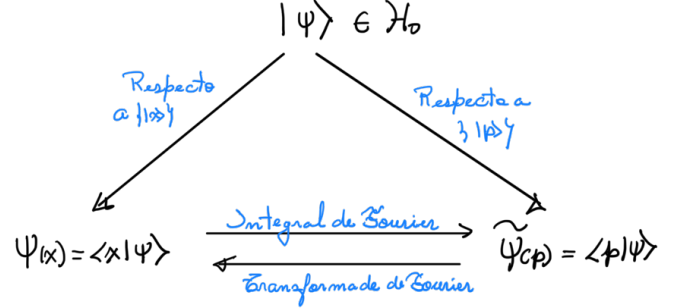
\includegraphics[scale=0.5]{img/transformadaFourier.png}
    \caption{Relación entre la base y la trasnformación usada para cambiar la función de estado de esta.}
    \label{fig:fourier}
\end{figure}

\begin{description}
    \item[Propiedad 14: ] $\mel{p}{X}{\psi} = i\hbar \displaystyle\pdv{\psim}{p}$. 
\end{description}



\section{Posición y Momentum 3-D}
Ahora estudiaremos los Observables de poisición y momentum en 3 dimensiones. Ya sabemos que la posición de las partículas está dada por $\vec{r} = (x,y,z)$ y $\vec{X} = (X,Y,Z)$.
\begin{tcolorbox}
        $$ X \ket{\vec{r}} = X \ket{\vec{x}} = X\ket{x,y,z} = x\ket{x,y,z} $$
        $$ Y \ket{\vec{r}} = Y \ket{\vec{y}} = Y\ket{x,y,z} = y\ket{x,y,z} $$
        $$ Z \ket{\vec{r}} = Z \ket{\vec{z}} = Z\ket{x,y,z} = z\ket{x,y,z}. $$
    También
        $$ \ket{\vec{r}} = \ket{x,y,z} = \ket{x} \ten \ket{y} \ten \ket{z} $$
        $$ \hilbert _1 = \hilbert _o \ten \hilbert _o \ten \hilbert _o. $$
\end{tcolorbox}
El conjunto de kets propios $\{ \ket{x,y,z} \}$ forma una base ortonormal $\hilbert _1$. Debido a que $\ket{\vec{x}}$ es una base ortonormal de $\hilbert _1$ tenemos que
    $$ \braket{\vec{x}}{\vec{x}'} = \delta ' (\vec{x} - \vec{x}'). $$
   

\subsection{Representación Respecto a $\{ \ket{\vec{x}} \}$}
Supongamos que la partícula está en el estado $\ket{\psi}\in \hilbert _1$. El ket $\pk$ se puede escribir como una superposición de los estados base.
    $$ \pk = \int _{\R ^3} \dd{^3  \vec{x}} \psi (\vec{x} \ket{\vec{x}}). $$
Debido a que $\{ \ket{\vec{x}} \}$ es una base ortonormal
    $$ \psi (\vec{x}) = \braket{\vec{x}}{\psi}. $$

\begin{description}
    \item[Propiedad 15: ] $[X_i ,X_j] = 0$ para $i,j = 1,2,3$. 
    \item[Propiedad 16: ] Siguiendo con la idea del operador traslación, tomando $a = \vec{a}$: $T_{\vec{a}}$ es unitario.
    \item 
\end{description}


\begin{definition}
    \textbf{Operador $P_j$:} \\
        $$ P_j = i\hbar \eval{\dv{T_{\vec{a}}}{a_j}} _{a_j = 0}. $$
    De esta definición se tiene
        $$ \mel{\vec{x}}{P_x}{\psi} = -i\hbar \pdv{\psi}{x} \qquad j = 1 $$
        $$ \mel{\vec{x}}{P_y}{\psi} = -i\hbar \pdv{\psi}{y} \qquad j = 2 $$
        $$ \mel{\vec{x}}{P_z}{\psi} = -i\hbar \pdv{\psi}{z} \qquad j = 3. $$
\end{definition}


\begin{description}
    \item[Propiedad 17: ] $[P_j,P_k] = 0 $.
    \item[Propiedad 18: ] $T_{\vec{a}} = e^{-\frac{i}{\hbar} \vec{a} \cdot \vec{P}}.$ 
    \item[Propiedad 19: ] Si $\vec{P} = (P_x,P_y,P_z)$ entonces
        $$ \mel{\vec{x}}{\vec{P}}{\psi} = -i\hbar \grad{\psi (\vec{x})}, $$
    donde $\psi (\vec{x}) = \braket{\vec{x}}{\psi}$.
    \item[Propiedad 20: ] Dado el momentum lineal total $P^2 = P_x ^2 + P_y ^2 + P_z ^2$. Entonces $\mel{\vec{x}}{P^2}{\psi} = -\hbar ^2 \laplacian{\psi}$.
    \item[Propiedad 21: ] $[X_j, P_k] = i\hbar \delta _{jk} I$. 
    \item[Propiedad 22: ] $[X_j ,P_j ^n] = i\hbar n P^{n - 1}$.
    \item[Propiedad 23: ] Sean $A,B,C$ operadores y $b,c$ números complejos.
        $$ [A,bB + cC] = b[A,B] + C[A,C]. $$
    \item[Propiedad 24: ] Sea $F(P_j) = \sum _{n=0} ^\infty a_n P_j ^n$ entocnes
        $$ [X_j ,F(P_j)] = i\hbar F' (P_j). $$
\end{description}


\section{Momentum Respecto a la Posición en 3-D}
El observable $\vec{P}$ es una terna ordenada (como era de esperarse luego de todo lo visto anteriormente) y son compatibles. Estos observables nos proporcionan una base ortonormal de nuestro espacio de estado. 

\begin{tcolorbox}
        $$ P_x \ket{\vec{p}} = P_x \ket{p_x,p_y,p_z} = p_x \ket{p_x,p_y,p_z} $$
        $$ P_y \ket{\vec{p}} = P_y \ket{p_x,p_y,p_z} = p_y \ket{p_x,p_y,p_z} $$
        $$ P_z \ket{\vec{p}} = P_z \ket{p_x,p_y,p_z} = p_z \ket{p_x,p_y,p_z}. $$
    También
        $$ \hilbert _1 = \hilbert _o \ten \hilbert _o \ten \hilbert _o. $$
\end{tcolorbox}

Sabemos
	$$ \psi (\vec{x}) = \braket{\vec{x}}{\psi}, $$
	$$ \psim (\vec{p}) = \braket{\vec{p}}{\psi}. $$

\begin{description}
	\item[Propiedad 25: ] $\braket{\vec{x}}{\vec{p}} = N e^{\frac{i}{\hbar} \vec{p} \cdot \vec{x}}$ Donde $N$ es una constante de normalización y $\vec{p} \cdot \vec{x} = xp_x + yp_y + zp_z$.
	\item[Propiedad 26: ] $\braket{\vec{x}}{\vec{p}} = \frac{1}{\qty(2\pi \hbar)^{3/2}} e^{\frac{i}{\hbar} \vec{p} \cdot \vec{x}}$.
	\item[Propiedad 27: (Transformada inversa de Fourier)] 
		$$ \psi (\vec{x}) = \frac{1}{\qty(2\pi \hbar)^{3/2}} \int _{\R^3} \dd{^3 \vec{p}} e^{\frac{i}{\hbar} \vec{p} \cdot \vec{x}} \psim (\vec{p}). $$
	\item[Propiedad 28: (Transformada de Fourier)] 
		$$ \psim (\vec{p}) = \frac{1}{\qty(2\pi \hbar)^{3/2}} \int _{\R^3} \dd{^3 \vec{p}} e^{-\frac{i}{\hbar} \vec{p} \cdot \vec{x}} \psi (\vec{x}). $$
\end{description}


\begin{definition}
	\textbf{Valor Propio Degenerado: } \\
	Sea $A:\hilbert \to \hilbert$ un opeardor lineal $a\in \C$ es un valor propio degenerado si y solo si existen vectores $\pk$ y $\ket{\phi}$ linealmente independientes tal que 
		$$ A\pk = a\pk $$
		$$ A\ket{\phi} = a\ket{\phi}. $$
	Recordemos del álgebra lineal que el conunto de todos los vectores propios de $A$ con valor propio $a$, forma un subespacio vectorial. De lo anterior tenemos que $a$ es un valor propio degenerado si y solamente si el espacio propio tiene dimensión mayor o igual a $2$.
\end{definition}


\begin{description}
	\item[Propiedad 29: ] Si $A$ y $B$ son observalbes que tienen la misma base ortonoral de kets porpios, entonces $A$ y $B$ son compatibles.
	\item[Propiedad 30: ] Si $A$ y $B$ son observables compatibles, donde todos sus valores propios son no degenerados, entonces $A$ y $B$ comparten base ortonormal de kets propios.
\end{description}

\begin{teorema}
	Si $A$ y $B$ son observables compatibles entonces $A$ y $B$ comparten base de kets propios.
\end{teorema}














\chapter{Energía y Hamiltoniano}








\chapter{Oscilador Armónico Cuántico}








\chapter{Espín $1/2$}










\chapter{Momentum Angular}



























%%%%
\part{Mecánica Clásica}

\vspace*{\fill}

\begin{center}
	\textit{''La frase más exitante que se puede oír en ciencia, la que anuncia nuevos descubrimientos, no es «eureka» sino «Eso es divertido...»'' - Isaac Asimov.}
\end{center}

\vspace*{\fill}

\chapter{Movimiento de una Partícula en una Dimensión}

Se estudiará el movimiento de una partícula a lo largo de una línea recta.

\section{Teoremas de Energía y Momentum}
El movimiento de una partícula esta gobernado por la ecuación de la Segunda Ley de Newton
\begin{equation}
	F = m\dv[2]{x}{t}.
\end{equation}

Antes de considerar su solución de esta ecuación es necesario recordar algunos conceptos básicos, como el momentum lineal
\begin{equation}
	p = mv = m\dv{x}{t}.
\end{equation}

Suponiendo que la masa es constante (esto no es cierto en casos específicos), se tiene

\begin{equation}
	F = \dv{p}{t}.
\end{equation}

Esta ecuación muestra que el cambio del momentum en el tiempo es igual a la fuerza aplicada. A esto le llamammos el Teorema del Momentum Lineal. Integrando en el tiempo, se tiene 
\begin{equation}
	p_2 - p_1 = \int _{t_1} ^{t_2} F \dd{t}.
\end{equation}

A la integral de la derecha se le conoce como \textit{Impulso}. \\


Otra cantidad importante a tomar en cuenta es la \textit{energía cinética}
\begin{equation}
	T = \frac{1}{2} mv^2.
\end{equation}

Multiplicando la Segunda Ley de Newton por la velocidad, se tiene lo siguiente
\begin{equation}
	\dv{t} \qty(\frac{1}{2} mv^2) = \dv{T}{t} = Fv.
\end{equation}
Integrando de ambos lados y reemplazando la velocidad por su definición, se llega al \textit{Teorema Trabajo y Energía}

\begin{equation}
	T_2 - T_1 = \int _{t_1} ^{t_2} F \dd{x}.
\end{equation}

\section{Fuerza}

\subsection{Fuerza Aplicada Dependiente del Tiempo}

SI la fuerza $F$ está dada por una función dependiente del tiempo, resolviendo el teorema impulso momento para $x$ y $\dot{x}$.
\begin{align}
	v &= v_o + \frac{1}{m} \int _{t_o} ^t F(t) \dd{t} \\
	x - x_o &= v_o (t - t_o) + \frac{1}{m} \int _{t_o} ^t \qty[\int _{t_o} ^t F(t) \dd{t}] \dd{t} .
\end{align}


\subsection{Fuerza de Restitución Dependiente de la Velocidad}
La Segunda Ley de Newton en términos de la velocidad
\begin{equation}
	m\dv{v}{t} = F(v).
\end{equation}
Integramos y se obtienen soluciones de la siguiente forma
\begin{align*}
	v &= \varphi \qty(v_o , \frac{t - t_o}{m}) \\
	x &= x_o + \int _{t_o} ^t \varphi \qty(v_o , \frac{t - t_o}{m}) \dd{t}.
\end{align*}
Estas fuerzas restitutivas dependen de potencias de la velocidad del objeto/sistema en movimiento 
	\begin{equation}
		F = \mp bv^n,
	\end{equation}
Si $n$ es un entero impar, se toma el signo negativo, en otro caso se toma el signo de modo que la velocidad sea opuesta a la velocidad.

\subsection{Fuerza Conservativa}

Para una fuerza dependiente exclusivamente de la posición. Ahora definimos la energía potencial
\begin{equation}
	V(x) = - \int _{x_s} ^x F(x) \dd{x}
\end{equation}
Con esto se puede definir la energía total
\begin{equation}
	E = T + V.
\end{equation}
Resolviendo para la velocidad se obtiene
\begin{equation}
	v = \dv{x}{t} = \sqrt{\frac{2}{m}} \qty[E - V(x)]^{1/2}
\end{equation}
entonces
\begin{equation}
	\sqrt{\frac{m}{2}} \int _{x_o} ^x \qty[E - V(x)]^{1/2} \dd{x} = t - t_o.
\end{equation}
Con todo esto obtenemos la relación directa entre potencial y fuerza
\begin{equation}
	F = -\grad{V}
\end{equation}

\subsubsection{Campos Vectoriales}
Para que un campo vectorial $\vec{F}$ sea considerado conservativo, deben cumplirse las siguientes condiciones:

\begin{enumerate}
    \item \textbf{Existencia de un potencial escalar:} Existe una función escalar $f$ tal que $\vec{F} = \nabla f$. Esto significa que el campo vectorial puede ser expresado como el gradiente de una función escalar.
    
    \item \textbf{La circulación de $\vec{F}$ sobre cualquier curva cerrada es cero:} Para que un campo vectorial $\vec{F}$ sea conservativo, la integral de línea del campo vectorial sobre cualquier curva cerrada $C$ debe ser cero:
    $$
    \oint_{C} \vec{F} \cdot d\vec{r} = 0
    $$
    Esto implica que el trabajo realizado por el campo a lo largo de una trayectoria cerrada es nulo.
    
    \item \textbf{Independencia del camino:} En un campo conservativo, la integral de línea de $\vec{F}$ entre dos puntos cualesquiera es independiente del camino tomado entre esos puntos. Es decir, si $A$ y $B$ son dos puntos en el espacio, entonces:
    $$
    \int_{A}^{B} \vec{F} \cdot d\vec{r}
    $$
    es la misma para cualquier camino entre $A$ y $B$.
    
    \item \textbf{La condición de rotacional cero (campo irrotacional):} Para un campo vectorial $\vec{F}$ ser conservativo, su rotacional debe ser cero en toda la región de interés:
    $$
    \nabla \times \vec{F} = \vec{0}
    $$
    Esta condición implica que no hay "vorticidad" en el campo vectorial.
    
    \item \textbf{Simplemente conexa del dominio:} Para que el criterio del rotacional cero garantice que un campo es conservativo, el dominio del campo debe ser simplemente conexo. Un dominio es simplemente conexo si cualquier curva cerrada dentro de él puede ser contraída continuamente a un punto sin salir del dominio. En otras palabras, no debe haber agujeros en el dominio.
\end{enumerate}



\subsection{Caída Libre}
Una situación más que conocida para nosotros, ahora le incluiremos fuerzas de resitución

\begin{equation}
	F = -mg - bv,
\end{equation}
Esta es una aproximación más didáctica que real, para objetos pequeños con velocidades terminales grandes, esta es una mejor aproximación
\begin{equation}
	F = bv^2.
\end{equation}



\section{Osciladores}

\subsection{Oscilador Armónico Simple}
\dsnote{Básico, bueno, bonito y barato, todos lo conocemos y nos gusta :3} La ecuación característica de los osciladores armónicos simple
\begin{equation}
	\ddot{x} + \omega _o ^2 x = 0.
\end{equation}
Cuya energía potencial y total es
\begin{align*}
	V(x) &= \frac{1}{2} kx^2 \\
	E &= \frac{1}{2} kA^2 
\end{align*}





\subsection{Diagramas de Fase}
Diagrama realizado con $x$ y $\dot{x}$ como las coordenadas. Estos diagramas muestran información reelevante acerca del movimiento del sistema. Estos diagramas tienen como objetivos
\begin{itemize}
	\item Visualización de la dinámica del sistema.
	\item Análisisd de estabilidad.
	\item Predicción del comportamiento futuro.
	\item Estudio de sistemas caóticos.
\end{itemize}


\subsection{Oscilaciones Amortiguadas}
El oscilador armónico simple es un oscilador libre. Para este tipo de oscilacion se tiene

\begin{equation}
	\ddot{x} + 2\beta \dot{x} + \omega _o ^2 x = 0.
\end{equation}
donde $\beta = b/2m$ es el parámetro de amortiguamiento. La solución general es la siguiente
\begin{equation}
	x(t) = e^{-\beta t} \qty[A_1 \exp{\sqrt{\beta ^2 - \omega _o ^2}t} + A_2 \exp{-\sqrt{\beta ^2 - \omega _o ^2}t}]
\end{equation}

Para este tipo de oscilaciones se tienen $3$ casos
\begin{description}
	\item[Subamortiguado: ] $\omega _o ^2 > \beta ^2$. Cuya solución es
		\begin{equation}
			x(t) = A e^{-\beta t} \cos{\omega _1 t - \delta} \qquad \omega _1 ^2 = \omega _o ^2 - \beta ^2.
		\end{equation}
	\item[Amortiguamiento Crítico: ] $\omega _o ^2 = \beta ^2$. Cuya solución es
		\begin{equation}
			x(t) = (A + Bt) e^{-\beta t}.
		\end{equation}
	\item[Sobreamortiguado: ] $\omega _o ^2 < \beta ^2$. Cuya solución es
		\begin{equation}
			x(t) = A e^{-\beta t} \qty[A_1 e^{\omega _2 t} + A_2 e^{-\omega _2 t}] \qquad \omega _2 = \sqrt{\beta ^2 - \omega _o ^2}.
		\end{equation}
\end{description}


\subsection{Oscilaciones Forzadas}
El caso más simple de oscilaciones forzadas es el de una fuerza externa senoidal
\begin{equation}
	F = -kx - b\dot{x} + F_o \cos{\omega t}.
\end{equation}

Matemáticamente se obtienen dos soluciones una complementaria y una partícular. La solución complementaria
\begin{equation}
	x_c (t) = e^{-\beta t} \qty[A_1 \exp{\sqrt{\beta ^2 - \omega _o ^2}t} + A_2 \exp{-\sqrt{\beta ^2 - \omega _o ^2}t}],
\end{equation}
y para la solución partícular
\begin{equation}
	x_p (t) = D \cos{\omega t - \delta}
\end{equation}

\dsnote{Revisando Thornton, p118}
\begin{align*}
	x_p (t) &= \frac{A}{\sqrt{(\omega _o ^2 - \omega ^2) + 4\omega ^2 \beta ^2}} \cos{\omega t - \delta} \\
	\delta &= \arctan{\frac{2\omega \beta}{\omega _o ^2 - \omega ^2}}.
\end{align*}













\chapter{Movimiento de una Partícula en Varias Dimensiones}

\section{Primeras y Segundas Derivadas en Diferentes Coordenadas}
Primera derivada en coordenadas esféricas
$$ \frac{d\vec{r}}{dt} = \dot{r} \hat{e}_r + r \left( \dot{\theta} \hat{e}_\theta + \dot{\phi} \sin\theta \, \hat{e}_\phi \right) $$

Segunda derivada en coordenadas esféricas
$$\frac{d^2\vec{r}}{dt^2} = \ddot{r} \hat{e}_r + \dot{r} \left( \dot{\theta} \hat{e}_\theta + \dot{\phi} \sin\theta \, \hat{e}_\phi \right) + r \left( \ddot{\theta} \hat{e}_\theta + \dot{\theta} \frac{d\hat{e}_\theta}{dt} + \ddot{\phi} \sin\theta \, \hat{e}_\phi + \dot{\phi} \cos\theta \dot{\theta} \, \hat{e}_\phi \right) $$

Primera derivada en coordenadas cilíndricas
$$ \frac{d\vec{r}}{dt} = \dot{\rho} \hat{e}_\rho + \rho \dot{\phi} \hat{e}_\phi + \dot{z} \hat{e}_z $$

Segunda derivada en coordenadas cilíndricas
$$ \frac{d^2\vec{r}}{dt^2} = \left( \ddot{\rho} - \rho \dot{\phi}^2 \right) \hat{e}_\rho + \left( \rho \ddot{\phi} + 2 \dot{\rho} \dot{\phi} \right) \hat{e}_\phi + \ddot{z} \hat{e}_z $$



\section{Osciladores Armónicos en Dos Dimensiones}
Considerando el movimiento de una partícula con dos grados de libertad.

\begin{equation}
	\left. \mqty{F_x = -kr\cos \theta = -kx \\ F_y = -kr\sin \theta = -ky} \right\} 
\end{equation}

Cuyas soluciones son
\begin{equation}
	\left. \mqty{x(t) = \cos{(\omega _x t - \alpha)} \\ y(t) = \cos{(\omega _y t - \beta)}} \right\}
\end{equation}
Las trayectorias seguidas por un oscilador en dos dimensiones se denominan \textit{figuras de Lissajous}.



\section{Teoremas del Momentum Angular}
El momentum angular está definido de la siguiente forma
\begin{equation}
L = rmv_\theta = mr^2 \dot{\theta}.
\end{equation}
Ahora, notemos que 
\begin{equation}
	\dv{L}{t} = \dv{t} (mr^2 \dot{\theta}) = rF_\theta
\end{equation}
Y de esto, integramos llegamos al \textit{Teorema Impulso-Momentum} para el momentum angular.
\begin{equation}
	L_2 - L_1 = mr_2 ^2 \dot{\theta} _2 - mr_1 ^2 \dot{\theta} _1 = \int _{t_1} ^{t_2} rF_\theta \dd{t}.
\end{equation}
Respecto a un punto $O$
\begin{equation}
	L_O = \vb{r} \cp \vb{p} = m\qty(\vb{r} \cp \vb{v}).
\end{equation}


\section{Movimiento en una Fuerza Central}
Las fuerzas centrales son aquellas que representan atracción ($F(r) < 0$) o repulsión ($F(r) > 0$) a un punto en concreto desde el origen. Normalmente son dos partículas interactuando. En la gran mayoría de los casos de fuerza central, dicha fuerza es inversamente proporcional al $r^2$. Bajo una fuerza central no se tiene torque, por ende
\begin{equation}
    \dv{L}{t} = 0.
\end{equation}
Con esto, se reduce el problema a dos ecuaciones diferenciales
\begin{align*}
    m\ddot{r} - mr\dot{\theta} ^2 &= F(r), \\
    mr\ddot{\theta} + 2m\dot{r} \dot{\theta} &= 0.
\end{align*}
Y sabiendo que la energía total es de la forma
\begin{equation}
    E = \frac{1}{2} m\dot{r} ^2 + \frac{1}{2} mr^2 \dot{\theta}^2 + V(r).
\end{equation}
Reemplazando el momentum angular,y despejando, se obtiene
\begin{align}
    \dot{r} &= \sqrt{\frac{2}{m}}\qty(E - V(r) - \frac{L^2}{2mr^2})^{1/2}, \\
    \sqrt{\frac{2}{m}} t &= \int _{r_o} ^r \frac{\dd{r}}{\qty(E - V(r) - \dfrac{L^2}{2mr^2})^{1/2}}, \\
    \theta &= \theta _o + \int _0 ^t \frac{L}{mr^2} \dd{t}.
\end{align}
Ahora, tomando la segunda ley de newton mostrada al inicio de la sección, reemplazamos el momentum angular
\begin{equation}
    m\ddot{r} = F(r) + \frac{L^3}{mr^3}.
\end{equation}
Esta ecuación tiene la forma del movimiento en una dimensión más una \textbf{fuerza centrífuga}. Esta es una \textit{fuerza ficticia}. Con esto, integrando, definimos el potencial efectivo
\begin{equation}
    'V(r)' = V(r) + \frac{L^2}{2mr^2}.
\end{equation}
El ultimo término es la energía potencial asociada a la fuerza centrífuga. 

\subsection{Fuerza Inversamente Proporcional al Cuadrado de la Distancia}
El problema más importante de la mecánica clásica es
    \begin{equation}
        F = \frac{K}{r^2} \vu{r} \qquad V(r) = \frac{K}{r}.
    \end{equation}
y el potencial efectivo
    \begin{equation}
        'V(r)' = \frac{K}{r} + \frac{L^2}{2mr^2}.
    \end{equation}

\section{Órbitas Elípticas, El Problema de Kepler}
Antes de los descubrimientos de Newton, Kepler anunció tres leyes del movimiento planetario dadas las observaciones astronomicas de Tycho Brahe.
\begin{enumerate}
    \item Los planetas se mueven en elipses con el sol en uno de los focos.
    \item Las áreas por las que pasa el radiovector desde el planeta al sol en tiempos iguales son iguales.
    \item El cuadrado del periodo de revolución es proporcional al cubo del semieje mayor.
\end{enumerate}





\chapter{Sistemas de Partículas}
\section{Leyes de Conservación}
\dsnote{Solo se enunciarán, no vale la pena la demostración.}
\subsection{Conservación del Momentum Lineal}
Es la segunda Ley de Newton, para varias dimensiones
\begin{equation}
    \dv{\vb{P}}{t} = 0.
\end{equation}

Y el centro de masa de un sistema de partículas se mueve como una única partícula cuya masa es la masa total del sistema, sobre la cual actúa una fuerza igual al total de las fuerzas externas actuando sobre el sistema.

\subsection{Conservación del Momentum Angular}
Se tiene
\begin{equation}
    \dv{\vb{L}}{t} = \vb{\tau}.
\end{equation}


\subsection{Conservación de la Energía}
Es una que ya vimos, se definió a principios de esta parte. 
\begin{align}
    E &= V + T,
\end{align}
donde $E$ es constante.





\section{Problema de los Dos Cuerpos}
Este es uno de los problemas más bonitos cuya solución es simple pero brutal. Tomaremos las dos partículas, las fuerzas entre ellas y las fuerzas externas
\begin{align*}
    m_1 \ddot{r} _1 &= F_1 ^i = F_1 ^i + F_1 ^e, \\
    m_2 \ddot{r} _2 &= F_2 ^i = F_2 ^i + F_2 ^e.
\end{align*}
Y se introduce un cambio de coordenadas en base al centro de masa y la distancia entre las partículas (\dsnote{No la distancia de cada una al centro de masa}).

\begin{align*}
    R &= \frac{m_1 r_1 + m_2 r_2}{m_1 + m_2} \\
    r &= r_1 - r_2.
\end{align*}
Cuya transformación inversa es
\begin{align*}
    r_1 &= R + \frac{m_2}{m_1 + m_2} r, \\
    r_2 &= R - \frac{m_1}{m_1 + m_2} r. 
\end{align*}
Entonces se tiene (asumiendo $F_1 ^e /m_1 = F_2 ^e /m_2$)
\begin{align*}
    M\ddot{R} &= F, \\
    \mu \ddot{r} &= F_1 ^i,
\end{align*}
donde $M = m_1 + m_2$, $\mu = \frac{m_1 m_2}{m_1 + m_2}$ (masa reducida). $F = F_1 ^e + F_2 ^e$ y $F_1 ^i$ es la fuerza de la partícula $2$ sobre la partícula $1$. \\

\dsnote{El problema de N cuerpos no es soluble analíticamente y la parte de Osciladores Acoplados se trabajará en la parte de mecánica lagrangiana y hamiltoniana.}



\chapter{Cuerpo Rígido}
Para un cuerpo macroscópico definimos la dendidad
\begin{equation}
	\rho = \dv{M}{V},
\end{equation}
con
\begin{equation}
	M = \iiint _{\text{cuerpo}} \rho \dd{V}.
\end{equation}

\section{Ubicación de un Cuerpo Rígido}
Se necesitan 6 coordenadas para describir la posición de un cuerpo rígido, para un punto $P_1$ $(x_1,y_1,z_1)$ (centro de masa), $(\theta _2, \phi _2)$ para la orientación de $P_2$ a una distancia de $P_1$ (un eje) y $\psi$ para la rotación alrededor del eje $P_1 P_2$.


Utilizando los teoremas de momentum lineal y rotacional se tiene que 
\begin{itemize}
	\item Si $F$ es independiente de la orientación, podemos resolver $F = M\ddot{R}$.
	\item Si $N$ es idnependiente de $R$, podemos resolver $\dv{L}{t} = N$.
	\item Si $F$ y $N$ dependen entre sí, las ecuaciones se resuelven acopladas.
\end{itemize}

\subsection{Consideraciones Generales}
Si el objeto gira alrededor de un punto arbitrario, $F = M\ddot{R}$ sirve para saber la fuerza necesaria que mantiene el punto fijo y $\dv{L}{t} = N$ nos da el movimiento de rotación. Aunque es dificil aplicar $\dv{L}{t} = N$ por la elección de los ángulos determinen la orientación del objeto.

\subsection{Momento de Inercia}
Tomando una partícula rotando alrededor de un eje
	\begin{equation}
		L = \sum _i m_i r_i ^2 \dot{\theta} = \qty(\sum _i m_i r_i ^2) \dot{\theta} = I_z \dot{\theta}
	\end{equation}
donde $I_z$ es el momento de inercia alrededor del eje $z$.
\begin{equation}
	I_z = \iiint _{\text{cuerpo}} \rho r^2 \dd{V}.
\end{equation}
\begin{itemize}
	\item Radio de giro: $Mk_z ^2 = I_z$, donde $k_z$ es la distancia de donde toda masa debe estar como partícula puntual para tener el mismo momento de inercia que el objeto original.
\end{itemize}

\subsection{Ecuación de Rotación}
Esta es la ecuación de movimiento para un cuerpo rígido alrededor de un eje fijo.
\begin{equation}
	\dv{L}{t} = I_z \ddot{\theta} = N_z.
\end{equation}


\subsection{Centro de Masa}
\begin{itemize}
	\item Si un cuerpo es simétrico respecto a un plano, el centro de masa está en el plano.
	\item Si un cuerpo es simétrico respcto de dos planos, el centro de masa está en la intersección de los planos.
	\item Si un cuerpo es simétrico alrededor de un eje, el centro de masa está en el eje.
	\item Si un cuerpo es simétrico respecto de tres planos, el centro de masa está en la intersección de los planos.
	\item \h{Importante: } Si un cuerpo se compone de varias partes cuyos centros de masa son conocidos, entonces el centro de masa del cuerpo compuesto se puede calcular como si las partes fueran partículas puntuales.
\end{itemize}

\begin{definition}
	\textbf{Centroide: } \\
	\begin{equation}
		R = \frac{1}{V} \iiint _V r\dd{V} \qquad R = \frac{1}{A} \iint _A r\dd{A} \qquad R = \frac{1}{s} \int _c r\dd{s}.
	\end{equation}
\end{definition}


\begin{teorema}
	\textbf{Teorema de Pappus: } Si una curva plana rota alrededor de un eje en el mismo plano y ambos no se interesectan, en el área de la superficie de revolución es igual a la longitud de la curva por la longitud de la trayectoria del centroide.
\end{teorema}




\begin{teorema}
	\textbf{Teorema de Ejes Paralelos: } El momento de inercia de un cuerpo alrededor de un eje dado es igual al momento de inercia alrededor de un eje paralelo que pasa por el centro de masa, más el momento de inercia alrededor del eje dado como si toda la masa del cuerpo estuviera concentrada en el centro de masa.
\end{teorema}



\begin{teorema}
	\textbf{Teorema de Ejes Perpendiculares: } Para una lámina plana, la suma de los momentos de inercia de una lámina plana alrededor de dos ejes perpendiculares en el plano de la lámina es igual al momento de inercia alrededor de un eje que pasa por el punto donde se intersectan, perpendicular a la lámina.
\end{teorema}




\chapter{Gravitación}
Ecuación de Gravitació Universal
\begin{equation}
	\vb{F} _{1\to 2} = \frac{Gm_1 m_2}{\abs{\vb{r}_1 - \vb{r}_2}^3} \qty(\vb{r}_1 - \vb{r}_2) = \iiint \frac{Gm (r' - r) \rho (r')}{\abs{r' - r}^3} \dd{V'} .
\end{equation}

Con esto se define el campo gravitacional
\begin{equation}
	g(r) = \iiint \frac{G (r' - r) \rho (r')}{\abs{r' - r}^3} \dd{V'}
\end{equation}
Y también se define la energía potencial gravitacional y el potencial gravitacional
\begin{equation}
	V_m (r) = \sum _i \frac{-Gmm_i}{\abs{r - r_i}} \qquad \mathcal{G} = \sum _i \frac{Gm_i}{\abs{r - r_i}}
\end{equation}
Los cuales cumplen con las siguientes relaciones, dado que la fuerza y el campo gravitacional son conservativos
\begin{equation}
	F = -\grad{V} \qquad g = \grad{\mathcal{G}}.
\end{equation}
por lo mismo
\begin{equation}
	\curl{g} = 0.
\end{equation}

Y utilizando lo que se verá para la Ley de Gauss en electricidad, aplicado aqui nos da como resultado, que el flujo gravitacional es
\begin{equation}
	\div{g} = -4\pi G\rho .
\end{equation}
y en términos del potencial
\begin{equation}
	\laplacian{\mathcal{G}} = -4\pi G\rho .
\end{equation}





\chapter{Sistema de Coordenadas en Movimiento}

Origen de coordenadas en movimiento
\begin{align*}
	r &= r^* + h \\
	r^* &= r - h .
\end{align*}
Los ejes de $O^*$ son paralelos a los de $O$, $O^*$ se mueve respecto a $O$.
\begin{align*}
	\dv{r}{t} &= \dv{r^*}{t} + \dv{h}{t}. \\
	a = a^* + a_h
\end{align*}

Al término $ma_h$ se le conoce como fuerza ficticia. Por segunda ley de newton
\begin{equation}
	m\dv[2]{r^*}{t} + ma_h = F
\end{equation}
Si $O^*$ se mueve con velocidad constante
	$$ m\dv[2]{r^*}{t} = F $$
Ahora para un sistema rotado
\begin{equation}
	r = x\vu{x} + y\vu{y} + z\vu{z} = x^* \vu{x^*} + y^* \vu{y^*} + z^* \vu{z^*}.
\end{equation}

Con todo esto se definen dos derivadas $\dv{^*}{t}$ para el sistema que rota y $\dv{t}$ para el sistema fijo. Definiremos un vetor $A$ en ambos sistemas de coordenadas
\begin{align*}
	A &= A_x \vu{x} + A_y \vu{y} + A_z \vu{z} \\
	A &= A_x ^* \vu{x}^* + A_y ^* \vu{y}^* + A_z ^* \vu{z}^*
\end{align*}

y encontramos sus derivadas respecto a su propio sistema de referencia
\begin{align*}
	\dv{A}{t} &= \dot{A}_x \vu{x} + \dot{A}_y \vu{y} + \dot{A}_z \vu{z} \\
	\dv{^* A}{t} &= \dot{A}_x ^* \vu{x}^* + \dot{A}_y ^* \vu{y}^* + \dot{A}_z ^* \vu{z}^* .
\end{align*}
Ahora, si queremos la derivada de $A$ en el sistema $O^*$
\begin{align*}
	\dv{A}{t} &= \dv{t} \qty[A_x ^* \vu{x}^* + A_y ^* \vu{y}^* + A_z ^* \vu{z}^*] \\
	&= \dot{A}_x ^* \vu{x}^* + \dot{A}_y ^* \vu{y}^* + \dot{A}_z ^* \vu{z}^* + A_x ^* \dv{\vu{x}^*}{t} + A_y ^* \dv{\vu{y}^*}{t} + A_z ^* \dv{\vu{z}^*}{t}.
\end{align*}
Supongamos que $O^*$ rota alrededor del eje $z$ con velocidad $\omega$ y consideremos un vector $B$ que está en reposo en $O^*$. Pero en $O$ tenemos que
	\begin{align*}
		\dv{B}{t} &= \omega B\sin \theta \vu{v} \\
		\dv{B}{t} &= \omega \cp B .
	\end{align*}

Desarrollando se llega al siguiente operador
\begin{equation}
	\dv{t} = \dv{^*}{t} + \omega \cp
\end{equation}

Y derivando nuevamente respecto al tiempo y reemplazando $A=r$
\begin{teorema}
	\textbf{Teorema de Coriolis: }
	\begin{equation}
		\dv[2]{r}{t} = \dv[2]{* r}{t} + 2\omega \times \dv{* r}{t} + \omega \times (\omega \times r) + \dv{* \omega}{t} \times r.
	\end{equation}
	donde el término $2\omega \times \dv{* r}{t}$ es la \textbf{aceleración de coriolis} y $\omega \times (\omega \times r)$ es la \textbf{aceleración centrípeta}. Y para una partícula cualquiera y una fuerza $F$ se tiene
	\begin{equation}
		\boxed{ m\dv[2]{*r}{t} = F + + m[g - \omega \times (\omega \times r)] - 2m\omega \times \dv{*r}{t}. }
	\end{equation}
	En donde al término $g_e = g(r) - \omega \times (\omega \times r)$ se le conoce como \textbf{gravedad efectiva}.
\end{teorema}

\section{Fuerza de Coriolis}
La ecuación para movimiento en la tierra es
\begin{equation}
	m\dv[2]{*r}{t} = F + + m[g - \omega \times (\omega \times r)] - 2m\omega \times \dv{*r}{t}.
\end{equation}
Dejando solo la fuerza de coriolis
	\begin{equation}
		m\dv[2]{*r}{t} = -2m\omega \times \dv{*r}{t}.
	\end{equation}

\begin{figure}[H]
	\centering
	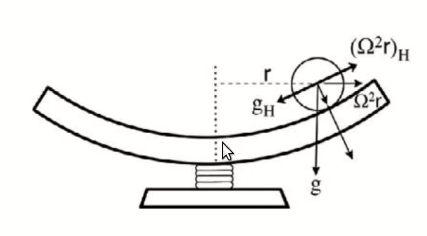
\includegraphics[scale=0.4]{./img/coriolis.png}
	\caption{Figura para ejemplificar la fuerza de \textit{Coriolis}.}
	\label{coriolis}
\end{figure}

Hacemos $\omega = (0,0,\omega)$ y llamamos $v = \dv{*r}{t} = (v_x, v_y, 0)$. Expandiendo el producto vectorial $ \dv{*}{t} (v_x,v_y,0) = (2\omega v_y,-2\omega v_x,0)$ entonces, se tienen ecuaciones diferenciales para las componentes
	\begin{equation}
		\dv{*v_x}{t} = 2\omega v_y, \qquad \dv{*v_y}{t} = -2\omega v_x.
	\end{equation}
Resolviendo las ecuaciones se tiene que 
	\begin{align*}
		v_y (t) &= A \cos{(2\omega t + \theta)} ,\\
		v_x (t) 6= A\sin{(2\omega t + \theta)}
	\end{align*}
Se tomarán como condiciones iniciales $v_x (0) = v_{x0}$ y $v_y (0) = 0$, entonces
	\begin{align}
		v_x (t) &= v_{x0} \sin{(2\omega t + \pi/2)} = \cos{(2\omega t)}, \\
		v_y (t) &= v_{x0} \cos{(2\omega t + \pi/2)} = \sin{(2\omega t)}.
	\end{align}
Integramos para encontrar la posición
	\begin{align}
		x(t) &= \frac{v_{x0}}{2\omega} \sin{(2\omega t)}, \\
		y(t) &= \frac{v_{x0}}{2\omega} \cos{(2\omega t)} - \frac{v_{x0}}{2\omega}.
	\end{align}
Es claro que la trayectoria de la partícula en el sistema estrellado es un círculo.

\subsection{Péndulo de Foucault}
Tomando un péndulo largo y pesado, esto nos da oscilaciones "planas" sin elevación. La fuerza de coriolis es perpendicular al plano de oscilación, es $<0.1\%$ de $mg_e$ y tiene un efecto de precesión del plano de oscilación. Para describir bien esto, nos 'iremos' a un sistema que rota con el plano de oscilación. \\

Introducimos coordenadas en donde el péndulo no precesa. Llamamos $\Omega \vu{z}$ a la \textit{velocidad de precesión del plano}. También llamamos $O'$ al sistema que gira con velocidad $\Omega \vu{z}$, recordamos cómo tomar las derivadas
\begin{equation}
	\dv{r}{t} = \dv{*r}{t} + \omega \times r,\qquad	\dv[2]{r}{t} = \dv[2]{* r}{t} + 2\omega \times \dv{* r}{t} + \omega \times (\omega \times r) + \dv{* \omega}{t} \times r
\end{equation}
Ahora transformaremos, nos trasladaremos del sistema $O^*$ al sistema primado, con lo que se tiene
\begin{equation}
	\dv{*r}{t} = \dv{\prime r}{t} + \Omega \vu{z} \times r, \qquad \dv[2]{*r}{t} = \dv[2]{\prime r}{t} + \Omega \vu{z}\times (\Omega \vu{z} \times r) + 2\Omega \vu{z} \times \dv{\prime r}{t}.
\end{equation}
\dsnote{Son 3 sistemas de coordenadas: El sistema fijo, el sistema estrellado que gira con el planeta y el sistema primado que es el que gira con el péndulo.} Ahora con un poco del álgebra y análisis vectorial\footnote{Identidad BAC-CAB: $\vb{A} \times (\vb{B} \times \vb{C}) = \vb{C}(\vb{A}\cdot \vb{C}) - \vb{C} (\vb{A} \times \vb{B})$} se llega a 
\begin{equation}
	m\dv[2]{\prime r}{t} = \tau + mg_e - 2m (\Omega \vu{z} + \omega) \times \dv{\prime r}{t} - m\Omega \qty[\Omega \vu{z} \cdot r + 2\omega \cdot r]\vu{z} + m(\Omega ^2 + 2\omega \cdot \Omega \vu{z}) r.
\end{equation}
El vector unitario $\vu{z}$ y el vector de posición $r$ están sobre el plano de oscilación. El vector resultante del producto cruz es el único que se sale del plano de oscilación y esto se escapa del objetivo del sistema primado; por ende, tenemos que ajustar la velocidad angular $\Omega$ para que todas las fuerzas involucradas estén dentro del plano de oscilación. Entonces es necesario que $\vu{z} \cdot (\Omega \vu{z} + \omega) = 0$, por lo tanto $\Omega = -\omega \cos{\theta}$ lo que contrarresta la precesión ocacionada por la fuerza de coriolis.





\section{Problema Restringido de los Tres Cuerpos}
Tomaremos el potencial para la masa $m$ del sistema de tres cuerpos
\begin{equation}
	V = -\frac{mM_1 G}{\qty[(x - x_1)^2 + y^2]^{1/2}} - \frac{mM_2 G}{\qty[(x - x_2)^2 + y^2]^{1/2}} - \frac{1}{2} m\omega ^2 \qty(x^2 + y^2),
\end{equation}
donde $\omega$ es la velocidad angular de la órbita circular $M_1$ y $M_2$, la cuál está dada por
	\begin{equation}
		\omega ^2 = \frac{(M_1 + M_2) G}{a^3}.
	\end{equation}
Al igual que las órbitas de fuerza central, nuestro análisis se basa en encontrar los puntos máximos y mínimos de la energía potencial.\\

Para hacer los cálculos más simples se realizará el siguiente cambio de variables.
\begin{align*}
	\xi = \frac{x}{a}, &\qquad \eta = \frac{y}{a}, \\
	\xi _1 = \frac{x_1}{a} = \frac{M_2}{M_1 + M_2}, &\qquad \xi _2 = \frac{x_2}{a} = -\frac{M_1}{M_1 + M_2} = \xi _1 - 1.
\end{align*}
Entonces, reemplazando variables
\begin{equation}
	V = \frac{m (M_1 + M_2) G}{a} \left\{ \frac{\xi _2}{\qty[(\xi - \xi _2)^2 + \eta ^2]^{1/2}} - \frac{\xi _1}{\qty[\qty(\xi - \xi _2)^2 + \eta ^2]^{1/2}} - \frac{1}{2} \qty(\xi ^2 + \eta ^2) \right\} .
\end{equation}

\subsection{Puntos Máximos y Mínimos}
La forma de proceder es tomar las derivadas de $V$ dada por la última ecuación respecto de $\xi$ y $\eta$ e igualarlas a cero. Cone esto llegamos a la siguiente relación
	\begin{equation}
		-\frac{\xi _2 (\xi - \xi _1)}{\abs{\xi - \xi _1}^3} + \frac{\xi _1 (\xi - \xi _2)}{\abs{\xi - \xi _2}^3} - \xi = 0.
	\end{equation}

Haciendo $\eta = 0$ se tienen $3$ puntos $(\xi _A ,0), (\xi _B ,0), (\xi _C ,0)$. Los siguientes dos puntos se encuentran con un poco de álgebra
\begin{align*}
	(\xi - \xi _2)^2 + \eta ^2 &= 1, \\
	(\xi - \xi _1)^2 + \eta ^2 &= 1.
\end{align*}
En donde los puntos $A,B,C$ son puntos silla y $D,E$ son máximos. El resto de la solución es gráfica.





\chapter{Mecánica del Medio Continuo}
\section{Cuerda Vibrante}
Consideraciones generales:
\begin{itemize}
	\item La vibración ocurre en el plano vertical.
	\item La longitud de la cuerda es $l$.
	\item La cuerda está fija en los extremos.
	\item La vibración es pequeña.
	\item Cada punto se mueve verticalmente.
	\item La tensión es constante.
\end{itemize}

Luego de realizar la deducción se tiene la ecuación de onda
\begin{equation}
	\laplacian{p} - \frac{1}{c^2} \pdv[2]{p}{t} = 0.
\end{equation}

Resolviendo la ecuación por separación de variables se tienen las siguientes ecuaciones
\begin{align}
	\Theta (t) &= A \cos{\omega t} + B \sin{\omega t}. \qquad \textbf{Ecuación de Helmholtz} \\
	X(x) &= C_x \cos{k_x x} + D_x + \sin{k_x x}, \\
	Y(y) &= C_y \cos{k_y y} + D_y + \sin{k_y y}, \qquad \textbf{Soluciones Espaciales} \\
	Z(z) &= C_z \cos{k_z z} + D_z + \sin{k_z z}.
\end{align}

Donde la constante de $z$ depende de las otras dos, y esta relación es
\begin{equation}
	\frac{\omega ^2}{c^2} = k_x ^2 + k_y ^2 + k_z ^2.
\end{equation}
Luego de aplicar las condiciones de frontera 
\begin{equation}
	p = \qty(A \cos{\omega _{lmn} t} + B \sin{\omega _{lmn} t}) \cos{\frac{l\pi x}{L_x}} \cos{\frac{m\pi y}{L_y}} \cos{\frac{n\pi z}{L_z}}.
\end{equation}

\begin{enumerate}
	\item Las frecuencias $\omega _{lmn}$ no son múltiplos enteros de una misma cantidad, como en el caso de la cuerda. Esto es importante porque es la razón por la cual una cuerda puede producir notas musicales.
\end{enumerate}

\subsection{Ondas Viajeras}
Luego de encontrar la solución a la ecuación de onda en una dimensión
\begin{equation}
	u(x,t) = A \sin{\frac{n\pi x}{l}} \cos{\frac{n\pi ct}{l}} + \sin{\frac{n\pi x}{l}} \sin{\frac{n\pi ct}{l}}.
\end{equation}


\subsubsection{Ondas Viajeras y Estacionarias}
\begin{equation}
	\underbrace{B \sin{\frac{n\pi x}{l}} \sin{\frac{n\pi ct}{l}}}_{\text{ONda Estacionaria}} = \underbrace{\frac{B}{2} \cos{\frac{n\pi}{l} (x - ct)}}_{\text{Onda Viajera a la }\to} - \underbrace{\frac{B}{2} \cos{\frac{n\pi}{l} (x + ct)}}_{\text{Onda Viajera a la } \leftarrow}.
\end{equation}

\begin{tcolorbox}
	Para formar una onda estacionaria tenemos que superponer dos ondas
viajeras con igual amplitud y que se muevan en direcciones opuestas con
igual velocidad. 
\end{tcolorbox}


\section{Equilibrio de Fluidos}
\subsection{Fuerzas de Volumen}
Fuerza de volumen $f$, es la traducción común de \textit{body force}. Es la fuerza que experimenta un fluido por unidad de volumen, de tal forma que un elemento de volumen $\dd{V}$ experimenta una fuerza dada por $f\dd{V}$. El ejemplo más común es la fuerza de volumen ejercida por la gravedad, que está dada como $f = \rho g$ donde $\rho$ es la densidad del fluido.

\subsection{Relación entre Presión y Energía Potencial}
Encontrar la presión dentro de un fluido en equilibrio sabiendo la fuerza de volumen $f(r)$ es equivalente a encontrar la \textbf{energía potencial} para una fuerza $F(r)$. Primero verificamos que  $\curl{f}$ sea cero en todo el fluido. Luego tomamos un punto  $r_1$ en donde la presión es conocida y utilizamos la expresión
	\begin{equation}
		p(r) = p_1 + \int _{r_1} ^r f\cdot \dd{r}.
	\end{equation}
que es una integral de línea a lo largo de una trayectoria. Si $\curl{f} = 0$ implica que $f$ se puede expresar como el gradiente de una cantidad. De la expresión entre la fuerza de volumen $f$ y la presión $p$ es
	$$ f = \grad{p}. $$
En el caso de fuerza de gravedad, sabemos que ésta apunta de arriba hacia abajo. El gradiente de la presión apunta en la misma dirección ya que la presión aumenta de arriba hacia abajo.



\section{Cinemática de Fluidos}
Se tienen dos puntos de vista
\begin{itemize}
	\item \textbf{Lagrangiano:} 
	\begin{itemize}
		\item Seguir el movimiento de un elemento de fluido.
		\item Dada su posición inicial $\to$ posición futura.
		\item Como un sistema de partículas, forma en la que describimos la cuerda.
	\end{itemize}
	\item \textbf{Euleriano:}
	\begin{itemize}
		\item Establecer densidad y velocidad para cada punto e instante.
		\item El fluido se describe con la densidad $\rho (x,y,z,t)$ y la velocidad $v(x,y,z,t)$.
		\item Centramos la atención en lo que sucede en un punto fijo en lugar de seguir a las partículas en su trayectoria.
	\end{itemize}
\end{itemize}


\subsection{Dos Tipos de Razones de Cambio}
Desarrollando un poco el diferencial de presión
\begin{equation}
	\boxed{ \dv{p}{t} = \pdv{p}{t} + v\cdot \grad{p}. }
\end{equation}

\subsection{Fluido Incompresible}
Estudiando un poco la divergencia se tiene
\begin{equation}
	\dv{t} (\delta V) = (\div{v}) \delta V.
\end{equation}
Un caso importante a considerar es cuando $\div{v} = 0$, en cuyo caso vemos de la derivada del volumen es igual a cero, o bien que $\delta V$ se mantiene constante. En otras palabras, decimos que el fluido es \textbf{incompresible}.

\begin{tcolorbox}
	Un fluido es incompresible si cumple con $\div{v} = 0$.
\end{tcolorbox}
Esta condición se cumple cuando el fluido es un líquido. Un gas se expande y se contrae, pero en ciertos casos se puede considerar incompresible también. Sin embargo, recordemos también que ningún objeto es totalmente líquido.

\subsection{Masa}
Suponiendo que la masa de un elemento de volumen es constante $\delta m = \rho \delta V$. Derivando respecto al tiempo y desarrollando $\dv{t} \delta m$
\begin{equation}
	\pdv{\rho}{r} + \div{\rho v} = 0,
\end{equation}
A lo que se le conoce como \textbf{ecuación de continuidad} y expresa e hecho de que la masa de cada elemento de volumen es constatne, por lo tanto la masa total de todo el fluido también es constante. En otras palabras, la masa se conserva.

\subsection{Voriticidad}
Es el elemento proyectado en la dirección de un vector unitario $\vu{n}$
\begin{equation}
	\text{Vorticidad} = \vu{n} \cdot \qty(\curl{v}).
\end{equation}
Si integramos la vorticidad en una superficie con vector normal, utilizando el teorema de Stokes, en donde si las integrales son cero podemos decir que la vorticidad es cero y esto nos dice que el fluido es \textbf{irrotacional}.

\subsection{Ecuacion de Movimiento para un Fluido Ideal}
\begin{equation}
	\pdv{v}{t} = v\cdot \grad{v} + \frac{1}{\rho} \grad{\rho} = \frac{f}{p}.
\end{equation}
Si $\rho = \rho (p)$ entonces el fluido es homogeneo.


\subsection{Ley de Conservación}
Vamos a partir de la ecuación de continuidad, la cual también le podemos llamar \textbf{ley de conservación de masa}. 

\begin{equation}
	\dv{t} \underbrace{\iiint _V \rho \dd{V}}_{\text{masa}} + \underbrace{\iint _S \vu{n} \cdot v \rho \dd{S}}_{\text{flujo de masa}} = 0.
\end{equation}
Esto dice que la forma de una ley de conservación es
\begin{equation}
	\dv{t} X + \text{flujo de } X = 0,
\end{equation}
donde $X$ es cualquier cantidad física qeu nos interese, por ejemplo: masa, momentum, energía, momentum angular, etc. Una forma generalizada es con la ecuación anterior es igual a $Q$, a la cual se le llama \textbf{fuente} o \textbf{sumidero}.\\

De esto y de la fuerza de volumen podemos concluir que 
\begin{equation}
	\frac{1}{2} \rho v^2 + p - \rho \mathcal{G} = \text{cte}.
\end{equation}

\subsection{Flujo Estacionario}
\begin{itemize}
	\item Velocidad, densidad, presión, fuerzas de volumen son constantes en el tiempo.
	\item No cambian en el tiempo pero si en e espacio.
	\item Las derivadas $\pdv{t}$ son cero.
	\item La expresión $\dv{t} = \pdv{t} + v\cdot \nabla \, \to \, \dv{t} = v\cdot \nabla$.
\end{itemize}






\chapter{Mecánica Lagrangiana y Hamiltoniana}

\section{Introducción}
¿Por qué esto no es satisfactorio en la física moderna?
\begin{enumerate}
	\item ''Oscurece'' algunas características de la dinámica de un sistema.
	\item No está clara la relación entre las leyes de Newton y la Mecánica Cuántica.
	\item Es dificil trabajar con sólidos.
\end{enumerate}

Identificar estructuras y simetrías en los sistemas. Sistemas locales: QED, QCD, Débiles.


\subsection{Mecánica Newtoniana}
Segunda ley de Newton
\begin{equation}
	\vec{F} = m\vec{a} \longrightarrow \vec{F} (\vec{r}, \dot{\vec{r}}) = \dot{\vec{p}}.
\end{equation}
donde $\dot{m} = 0$. Si conocemos $\vec{r}$ y $\dot{\vec{r}}$ en un tiempo $t=t_o$, integrando se encuentra $\vec{r} (t)$.

\subsection{Marco de Referencia Inercial}
Es en el que una partícula con masa constante viaja en una línea recta.
\begin{equation}
	\vec{r} = \vec{r}_o + \vec{v} t.
\end{equation}
Si $S$ es un marco de referencia inercial se tienen $10$ transformaciones lineales independientes $S \to S\prime$ también es un M.R. inercial.
\begin{itemize}
	\item 3 Rotaciones: $\vec{r}' = O \vec{r}$ donde $O$ es una matriz $3\times 3$ ortogonal.
	\item 3 Traslaciones: $\vec{r}' = \vec{r} + \vec{c}$ donde $\vec{c}$ es un vector constante.
	\item 3 Boost: $\vec{r}' = \vec{r} + \vec{u} t$ donde $\vec{u}$ es una velocidad constante.
	\item 1 Traslaciones Temporales: $t' = t + c$ donde $c$ es real y constante.
\end{itemize}
Las leyes de Newton son invariantes ante este grupo de transformaciones: \textbf{Grupo Galileano.}


\subsection{Momento Angular}
\begin{equation}
	\vec{L} = \vec{r} \times \vec{p}
\end{equation}
Medimos respecto a un punto en partícular.
\begin{equation}
	\vec{\tau} = \dot{\vec{L}}
\end{equation}

\subsubsection{Leyes de Conservación}
\begin{itemize}
	\item Si $\vec{F} = 0$ entonces $\vec{p}$ es constante.
	\item Si $\vec{\tau} = 0$ entonces $\vec{L}$ es constante.
\end{itemize}

\subsection{Energía}
Energía cinética $T = \frac{1}{2} m \dot{\vec{r}} \cdot \dot{\vec{r}}$
\begin{equation}
	\dv{T}{t} = \vec{F} \cdot \dot{\vec{r}},
\end{equation}
entonces
\begin{equation}
	W = \int _{r_1} ^{r_2} \vec{F} \cdot \dd{\vec{r}}.
\end{equation}

\textbf{Fuerzas Conservativas:} El trabajo realizado es independiente de la trayectoria. Y para una trayectoria cerrada
\begin{equation*}
	\oint \vec{F} \cdot \dd{r} = 0 \quad \Leftrightarrow \quad \curl{\vec{F}} = 0.
\end{equation*}
Por lo que se puede escribir $\vec{F} = -\grad{V(r)}$. \\

Energía cinética de un sistema $T = \frac{1}{2} \sum _i m \dot{\vec{r}}_i ^2$ y tomando $\vec{r} _i = \vec{R} + \vec{\rsim}$
\begin{equation}
	T = \frac{1}{2} M \dot{\vec{R}}^2 + \frac{1}{2} \sum _i \dot{\vec{\sim}},
\end{equation}
como en el caso de una sola partícula
\begin{equation}
	T(t_2) - T(t_1) = \sum _i \int \vec{F} _i ^{ext} \cdot \dd{\vec{r}_i} + \sum_{i\neq j} \int \vec{F} _{ij} \cdot \dd{\vec{r}_i}.
\end{equation}

\begin{itemize}
	\item Fuerzas externas conservativas: $\vec{F} _i ^{ext} = -\grad{V_i} \qty(\vec{r}_1, \ldots ,\vec{r}_N)$.
	\item Fuerzas internas conservativas: $\vec{F}_{ij} = -\nabla _i V_{ij} (\vec{r}_1 ,\ldots ,\vec{r}_N)$. $\vec{F} _{ij} = -\vec{F}_{ij}$ $\to$ $V_{ij} = V_{ji}$ entonces $V_{ij} (\vec{r}_1 ,\ldots ,\vec{r}_N) = V_{ij} (\abs{\vec{r}_1 - \vec{r}_j})$.  
\end{itemize}

\begin{equation}
	T(t_2) - T(t_1) = -\sum _i \int \nabla _i V_i (\vec{r}_i) \cdot \dd{r}_i - \sum _{i\neq j} \int \nabla _i V_{ij} (r_1 ,\ldots, r_N) \cdot \dd{r}_i.
\end{equation}


\section{Generalidades}
\subsection{Principio Variacional y Ecuación de Lagrange}
Movimiento de un sistema. Coordenadas generalizadas: $q_1 ,q_2, \ldots, q_n$, espacio de $n$ dimensiones \dsnote{Espacio de Configuración}\footnote{Cada punto de la curva en el espacio de configuración es un instante en la configuración del sistema.}. 

\subsection{El Principio de Hamilton (Principio de Mínima Acción)}
El movimiento del sistema de un tiempo $t_1$ a un tiempo $t_2$ es tal que la acción
	\begin{equation}
		I = \int _{t_1} ^{t_2} \lagran \dd{t}
	\end{equation}

donde $\lagran$ es el Lagrangiano $T - V$, tiene un valor estacionario para el movimiento.
\begin{align*}
	\delta I &= 0, \\
	\delta I &= \delta \int _{t_1} ^{t_2} \lagran (q_1 ,\ldots ,q_n ,\dot{q}_1 ,\ldots ,\dd{q}_n ;t) \dd{t} = 0.
\end{align*}
Principio de Hamilton es suficiente para derivar las ecuaciones de movimiento.

\subsection{Cálculo de Variaciones}
\dsnote{''Repaso'' de algo que nunca se vió bien xd.}
Consideremos un problema de $1$ dimensión $f(y,\dot{y} ,x)$ donde $y = y(x)$, $\dot{y} = \dv{y}{x}$, $[x_1 ,x_2]$. Todo esto es por $\delta J = 0$, entonces
	\begin{equation}
		J = \int _{x_1} ^{x_2} f(y,\dot{y},t) \dd{x}.
	\end{equation}
Donde $y(x,\alpha)$ son posibles trayectorias y $y(x,0)$ es la trayectoria correcta. Podemos escribir $y(x,\alpha) = y(x,0) + \alpha \eta (x)$, donde $\eta (x)$ tiene que ser $0$ en $x_1$ y $x_2$. 
\begin{align*}
	J(\alpha) = \int _{x_1} ^{x_2} f\qty(y(x,\alpha), \dot{y} (x,\alpha), x) \dd{x}, \\
	\qty(\dv{J}{\alpha}) _{\alpha = 0} = 0. \qquad \text{Para un punto estacionario.}
\end{align*}

Derivando
\begin{equation}
	\dv{J}{\alpha} = \int _{x_1} ^{x_2} \qty(\pdv{f}{y} \pdv{y}{\alpha} + \pdv{f}{\dot{y}} \pdv{\dot{y}}{\alpha}) \dd{\alpha}
\end{equation}
Considerando solo la segunda derivada al realizar integración por partes
\begin{equation}
	\int _{x_1} ^{x_2} \pdv{f}{\dot{y}} \pdv{\dot{y}}{\alpha} \dd{x} = \int _{x_1} ^{x_2} \pdv{f}{\dot{y}} \pdv[2]{y}{\alpha}{x} \dd{x} = - \int _{x_1} ^{x_2} \dv{x} \qty(\pdv{f}{\dot{y}}) \pdv{y}{\alpha} \dd{x}.
\end{equation}

\begin{align*}
	\dv{J}{\alpha} &= \int _{x_1} ^{x_2} \qty(\pdv{f}{y} - \dv{x} \pdv{f}{\dot{y}}) \pdv{y}{\alpha} \dd{x} \\
	&\int _{x_1} ^{x_2} \qty(\pdv{f}{y} - \dv{x} \pdv{f}{\dot{y}}) \qty(\pdv{y}{\alpha})_{\alpha = 0} \dd{x} = 0 \qquad \text{Condición puntos estacionarios} \\
	\text{Recordemos } &\quad y(x,\alpha) = y(x,0) + \alpha \eta (x).
\end{align*}

\subsubsection{Lema: }
\begin{equation}
	\int _{x_2} ^{x_1} M(x) \eta (x) \dd{x} = 0
\end{equation}
para $\eta (x)$: función arbitraria y continua (hasta la segunda derivada). $M(x)$ se desvanece en el intervalo $(x_1,x_2)$
\begin{equation}
	\pdv{f}{y} - \dv{x} \qty(\pdv{f}{\dot{y}}) = 0
\end{equation}
la cantidad diferencial
	\begin{equation}
		\qty(\pdv{y}{\alpha})_{\alpha = 0} \dd{\alpha} \equiv \delta y
	\end{equation}
variación infinitesimal de la trayectoria variada respecto de la trayectoria correcta. La variación de $J$
\begin{equation}
	\qty(\pdv{J}{\alpha})_{\alpha = 0} \dd{\alpha} \equiv \delta J
\end{equation}
entonces
\begin{equation}
	\delta J = \int _{x_1} ^{x_2} \qty(\underbrace{\pdv{f}{y} - \dv{x} \pdv{f}{\dot{y}}}_{=0}) \delta y \dd{x} = 0
\end{equation}

\subsection{Principio de Hamilton y Ecuación de Lagrange}
\begin{equation}
	\delta J = \int _1 ^2 f(y_1 (x), \ldots; \dot{y} _1 (x), \ldots; x) \dd{x}
\end{equation}
Lo de $y_i(x,\alpha)$ se cumple para todas las $i$, donde lo que nos interesa son las $y_i (x,0)$, sabiendo que $\eta _i (x)$ se desvanecen en los extremos. Realizando el mismo análisis que se realizó en la subsección anterior, se llega a 
	\begin{equation}
		\boxed{ \pdv{f}{y_i} - \dv{x} \pdv{f}{\dot{y}_i} = 0 }
	\end{equation}
En donde si se tienen $N$ partículas, implica tener $n = 3N$ coordenadas. Cambiando de coordenadas
\begin{equation}
	\boxed{ \dv{t} \pdv{\lagran}{\dot{q}_i } - \pdv{\lagran}{q_i} = 0 }
\end{equation}
a lo que se conoce como \textbf{Ecuación de Lagrange}.

\subsection{Restricción en las Coordenadas Generalizadas}

\subsubsection{Restricciones Holonómicas}
\begin{equation}
	f(x_A ,t) = 0
\end{equation}
$\alpha = 1,2,\ldots ,N-n$ con $N$ número total de coordenadas y $n$ número de grados de libertad. Por ejemplo: para $M$ partículas, se tienen $3M$ ecuaciones, que es lo mismo que $3M = N$ coordenadas, y $n$ ecuaciones/grados de libertad.
\paragraph{Multiplicadores de Lagrange} $x_A = x_A (q_1, \ldots ,q_n)$, $N - n$ nuevos grados dinámicos de libertad, $\lambda _\alpha (t)$. Definimos el nuevo lagrangiano $\lagran ^\prime = \lagran (x^A, \dot{x}^A) + \lambda _\alpha f_\alpha (x^A ,t)$
\begin{equation}
	\underbrace{\dv{t} \pdv{\lagran}{\dot{x}_A} - \pdv{\lagran}{x_A}}_{\text{La ecuación de movimiento sin restricciones}} = \underbrace{\lambda _\alpha \pdv{f_\alpha}{x_A}}_{Restricciones en el sistema}
\end{equation}

\begin{teorema}
	\begin{equation}
		\lagran [q_i, \dot{q}_i,t] = \lagran [x^A(q_i ,t), \dot{x}^A (q_i ,\dot{q}_i ,t),t]
	\end{equation}
	Imponer una restricción $\lagran ^\prime = \lagran + \lambda _\alpha f_\alpha$
	\begin{equation}
		\boxed{ \dv{t} \pdv{\lagran}{\dot{q}_i} - \pdv{\lagran}{q_i} = \lambda _\alpha \pdv{f_\alpha}{q_i}, } \qquad \to \qquad \boxed{ \pdv{f_\alpha}{q_i} = 0. }
	\end{equation}
\end{teorema}
\paragraph{Resumen} Un sistema descrito por $N$ coordenadas generalizadas $q_i$
\begin{align*}
	\lagran (q_i ,\dot{q}_i ,t) \to \dv{t} \pdv{\lagran}{\dot{q}_i} - \pdv{\lagran}{q_i} = 0.
\end{align*}
\begin{itemize}
	\item Momento conjugado de $q_i$ $/$ momento canónico
	\begin{align}
		p_i &= \pdv{\lagran}{\dot{q}_i} \\
		\boxed{ \dot{p}_i = \pdv{\lagran}{q_i}. }
	\end{align}
\end{itemize}

\subsection{Teorema de Noether}
\begin{definition}
	$F(q_i, \dot{q}_i, t)$ constante de movimiento, cantidad conservada.
	\begin{equation}
		\dv{F}{t} = 0 \qquad \sum _{j=1} ^N \qty(\pdv{F}{q_j} \dot{q}_j + \pdv{F}{\dot{q}_i} \ddot{q}_i) + \pdv{F}{t} = 0
	\end{equation}
	para $q_i$ que satisface la ecuación de movimiento. Si $\lagran$ no depende explícitamente del tiempo.
	\begin{equation}
		H = \sum _j \dot{q}_j \pdv{\lagran}{\dot{q}_j} - \lagran = \text{cte}.
	\end{equation}
	Derivando el Hamiltoniano respecto al tiempo se supone $\pdv{\lagran}{q_j} = 0$ solo para algunas $q_j$.
	\begin{align*}
		p_j &= \pdv{\lagran}{\dot{q}_j} \\
		\dv{p_j}{t} &= \dv{t} \pdv{\lagran}{\dot{q}_j} = \pdv{\lagran}{q_j} = 0.
	\end{align*}
	Mapeo de los parametros $q_j = Q_j (s,t)$ $s\in \R$ De modo que $q_j (t) = Q_j (0,t)$, se dice que esta transformación es una simetría contínua del $\lagran$.
	\begin{equation}
		\pdv{\lagran}{s} (Q_j (s,t), \dot{Q}_j (s,t)) = 0.
	\end{equation}
	El teorema de Noether: Para cada una de estas simetrías hay una cantidad conservada.
	\begin{align*}
		\pdv{\lagran}{s} &= \pdv{\lagran}{Q_j} \pdv{Q_j}{s} + \pdv{\lagran}{\dot{Q}_j} \pdv{\dot{Q}_j}{s} \\
		\eval{\pdv{\lagran}{\dot{q}_j} \pdv{Q_j}{s}}_{s=0} &= \text{cte}.
	\end{align*}
	\begin{itemize}
		\item Invarianza de $\lagran$ ante traslaciones: Se conserva el momentum lineal.
		\item Invarianza de $\lagran$ ante rotaciones: Se conserva el momentum angular.
		\item Homogeneidad en el tiempo: Conservaciń de la energía.
	\end{itemize}
\end{definition}

\section{Formalismo de Hamilton}

\subsection{Ecuación de Hamilton}
\begin{equation}
	H(q_i, p_i, t) = \sum _{i=1} ^n p_i q_i - \lagran (q_i,p_i,t)
\end{equation}
con $\pdv{\lagran}{\dot{q}_i} = p_i$, ahora veamos la variación de $H$
\begin{equation}
	\dd{H} = (\dd{p}_i) \dot{q}_i - \pdv{\lagran}{q_i} \dd{q}_i - \pdv{\lagran}{t} \dd{t}
\end{equation}
Esto lo podemos escribir como
\begin{align}
	\dd{H} &= \pdv{H}{q_i} \dd{q}_i + \pdv{H}{p_i} \dd{p}_i + \pdv{H}{t} \dd{t} \\
	\boxed{\dot{p}_i = -\pdv{H}{q_i}} &\qquad \boxed{\dot{q}_i = \pdv{H}{p_i}} \qquad \boxed{-\pdv{\lagran}{t} = \pdv{H}{t}}.
\end{align}




\subsection{Teorema de Liuville}







\subsection{Brakets de Poisson}
Teniendo $f(p,q)$, $g(q,p)$ se define un braket de poisson
\begin{equation}
	\{ f,g \} = \pdv{f}{q_i} \pdv{g}{p_i} - \pdv{f}{p_i} \pdv{g}{q_i}.
\end{equation}
Con las siguientes propiedades
\begin{itemize}
	\item $\{ f,g \} = -\{ g,f \}$.
	\item Linealidad: $ \{ \alpha f + \beta g, h \} = \alpha \{ f,h \} + \beta \{ g,h \} $.
	\item Leibniz rule: $\{ fg,h \} = f\{ g,h \} + \{ f,h \} g$.
	\item Identidad de Jacobi: $\{ f,\{ g,h\} \} + \{ g,\{ h,f\} \} + \{ h,\{ f,g\} \} = 0$.
	\item Y por ultimo, para una función:
		\begin{equation}
			\dv{f}{t} = \{ f,H \} + \pdv{f}{t}.
		\end{equation}
\end{itemize}




\subsection{Transformaciones Canónicas}
Tomando $\mathcal{J} _{ij} \equiv \pdv{y_i}{x_j}$, para que las ecuaciones de Hamilton queden invariantes
	\begin{equation}
		\boxed{ \mathcal{J} J \mathcal{J} ^T = J.} \qquad \text{Transformación Canónica.}
	\end{equation}

\begin{teorema}
	Los brackets de Poisson son invariantes ante transformaciones canónicas. Si los brackets de Poisson preservan la estructura:
	\begin{equation}
		\{ Q_i,Q_j \} = 0 \qquad \{ P_i,P_j \} = 0 \qquad \{ Q_i,p_j \} = \delta _{ij}
	\end{equation}
	la transformación es canónica.
\end{teorema}
















\chapter{Cuerpo Rígido}
\section{Generalidades}
$N$ puntos en donde la distancia entre ellos está fijo $\abs{r_i - r_j} = $constante en el límite continuo $\sum _i m_i \to \int \dd{r} \rho (r)$. En donde se tienen $6$ grados de libertad $3$ traslaciones y $3$ rotaciones. Ahora definimos $\{ \vu{\overset{\sim}{e}}_a \}$ es el marco de referencia del espacio y $\{ \vu{e}_a \}$ es el marco de referencia del cuerpo rígido. En donde los productos internos entre elementos de los marcos de referencia cumplen con la ortonormalidad. \\

Espacio de configuración, $C$, matrices $3\times 3$ ortogonales especiales SO($3$).

\subsection{Velocidad Angular}
Teniendo $\vec{r} (t) = \overset{\sim}{r} _a (t) \vu{\overset{\sim}{e}_a} = r_a \vu{e} _a (t)$, ahora $r_a \vu{e} _a (t) = r_a R_{ab} (t) \vu{\overset{\sim}{e}} _b$, donde $R_{ab}$ son elementos de una matriz. Derivamos respecto al tiempo con lo que analizamos tanto los vectores posición como la base $\dv{\vu{e}_a (t)}{t} = \dv{R_{ab}}{t} R_{cd} \vu{e}_a = \omega _{ac} \vu{e}_c$ y por facilidad definimos un objeto con un solo índice $\omega _a = \frac{1}{2} \varepsilon _{abc} \omega _{bc}$\footnote{Donde $\varepsilon _{abc}$ es conocido como el símbolo de Levi Civita.}.
\begin{equation}
	\dv{\vu{e}_a}{t} = \vec{\omega} \times \vu{e}_a.
\end{equation}
con $\omega$ velocidad angular instantánea en el marco de referencia del cuerpo rígido.



\subsection{El Tensor de Inercia}
\begin{equation}
	T = \frac{1}{2} \sum _i m_i \dot{\vec{r}}_i ^2
\end{equation}
usando $\dot{\vec{r}} = \vec{\omega} \times \vec{r}$
\begin{equation}
	T = \frac{1}{2} \sum _i m_i (\vec{\omega} \times \vec{r}_i) \times (\vec{\omega} \times \vec{r} _i)
\end{equation}
usando y desarrollando una identidad para los producto cruz e interno, por lo que se tiene que
\begin{equation}
	T = \frac{1}{2} \omega _a I_{ab} \omega _b,
\end{equation}
donde $I_{ab} = \sum_i m_i \qty[\vec{r}_i \cdot \vec{r}_i \delta _{ab} - (\vec{r}_i)_a (\vec{r}_i)_b]$ donde $I_{ab}$ es el tensor de inercia, es simétrico
\begin{equation}
	I = \int \dd ^3 r \rho (\vec{r}) \mqty( y^2 + z^2 & -xy & -xz \\ -xy & x^2 + z^2 & -yz \\ -xz & -yz & y^2 + x^2 )
\end{equation}

$I^\prime = OIO^T$ donde $I^\prime$ es diagonal $I^\prime = \mqty(\dmat{I_1,I_2,I_3})$ con $I_a$ son los momentos de inercias principales.

\begin{tcolorbox}
	Propiedades del cuerpo rígido están dadas por su masa, su momento de inercia y sus ejes principales.
\end{tcolorbox}

$I_a$ es real y positivo.
\begin{equation}
	I_{ab} c^a c^b = \sum _i \qty(r_i ^2 c^2 - (\vec{r}_i \cdot \vec{c})^2) \geq 0.
\end{equation}
Si $\vec{c}$ es autovector de $I$, $I_{ab} c_a c_b = I_a \abs{\vec{c}}^2$, $I_a > 0$.

\begin{teorema}
	\textbf{Teorema de Ejes Paralelos: (Forma tensorial)}
	\begin{equation}
		\boxed{ \qty(I_c)_{ab} = \qty(I_{cm})_{ab} \qty(c^2 \delta _{ab} - c_a c_b)M }.
	\end{equation}
\end{teorema}


\subsubsection{Ecuaciones de Euler}
\begin{align*}
	I_1 \dot{\omega}_1 + \omega _2 \omega _3 (I_3 - I_2) &= 0, \\
	I_2 \dot{\omega}_2 + \omega _1 \omega _3 (I_1 - I_3) &= 0, \\
	I_3 \dot{\omega}_3 + \omega _1 \omega _2 (I_2 - I_1) &= 0.
\end{align*}


















































































%%%%%
\chapter{Electromagnetismo}
\part{Reducción de Datos}
\chapter{Materia Condensada}
%\input{general.tex}


%\bibliographystyle{abbrv}
%\bibliography{references}
\end{document}


